\documentclass[11pt,a4paper]{article}

% ==================================================================
%  Typography and layout
% ==================================================================
\usepackage[T1]{fontenc}
\usepackage[sc]{mathpazo}
\usepackage[top=1in,bottom=0.8in,left=1in,right=1in,headheight=14pt]{geometry}
\usepackage{setspace}
\setstretch{1.15}
\usepackage[final]{microtype}

\usepackage{amsmath,amssymb,mathtools,bm}
\usepackage{amsthm,thmtools}
\usepackage{booktabs,array}
\usepackage[font=small,labelfont=sc,labelsep=period,skip=6pt]{caption}
\usepackage{enumitem}
\usepackage{xcolor}
\usepackage[most]{tcolorbox}
\usepackage{titlesec}
\usepackage{fancyhdr}
\usepackage{etoolbox}
\usepackage{tikz}
\usetikzlibrary{arrows.meta}
\usepackage{pgfplots}
\pgfplotsset{compat=1.17}
\usepackage[colorlinks=true,linkcolor=black!75!blue,citecolor=black,urlcolor=black!75!blue]{hyperref}

\allowdisplaybreaks[2]
\renewcommand{\arraystretch}{1.35}
\setlist{itemsep=3pt,topsep=5pt,leftmargin=1.6em}

% section styles
\titleformat{\section}{\Large\bfseries}{\thesection}{0.9em}{}
\titlespacing*{\section}{0pt}{4ex plus 1ex minus .5ex}{2.2ex plus .4ex}
\titleformat{\subsection}{\large\bfseries}{\thesubsection}{0.8em}{}
\titlespacing*{\subsection}{0pt}{3.4ex plus 1ex minus .4ex}{1.4ex plus .3ex}
\titleformat{\paragraph}[runin]{\normalsize\bfseries}{}{}{}[.]
\titlespacing*{\paragraph}{0pt}{2ex plus .5ex minus .3ex}{0.6em}

% running heads
\pagestyle{fancy}
\fancyhf{}
\renewcommand{\sectionmark}[1]{\markboth{\thesection\enspace #1}{}}
\fancyhead[L]{\small\scshape\nouppercase{\leftmark}}
\fancyhead[R]{\small\thepage}
\renewcommand{\headrulewidth}{0.3pt}

% ==================================================================
%  Theorem-like environments
% ==================================================================
\declaretheoremstyle[spaceabove=9pt,spacebelow=9pt,headfont=\bfseries,bodyfont=\itshape,notefont=\normalfont\bfseries,notebraces={(}{)}]{thm}
\declaretheoremstyle[spaceabove=9pt,spacebelow=9pt,headfont=\bfseries,bodyfont=\normalfont,notefont=\normalfont\bfseries,notebraces={(}{)}]{defn}
\declaretheorem[style=thm,name=Theorem,numberwithin=section]{theorem}
\declaretheorem[style=thm,name=Proposition,sibling=theorem]{proposition}
\declaretheorem[style=thm,name=Lemma,sibling=theorem]{lemma}
\declaretheorem[style=defn,name=Definition,sibling=theorem]{definition}
\declaretheorem[style=defn,name=Example,sibling=theorem]{example}
\declaretheorem[style=defn,name=Assumption,numberwithin=section]{assumption}
\declaretheorem[style=defn,name=Assumptions,numbered=no]{asmset}

% "Why" boxes: a quiet left rule, no ornament
\newtcolorbox{whybox}[1]{enhanced,breakable,
  colback=black!2.5,colframe=black!2.5,boxrule=0pt,arc=0pt,
  left=11pt,right=9pt,top=7pt,bottom=7pt,
  borderline west={1.3pt}{0pt}{black!60},
  before skip=13pt,after skip=13pt,
  before upper={{\scshape Why}\;\;\textit{#1}\par\vspace{4pt}}}

% ==================================================================
%  Notation
% ==================================================================
\newcommand{\E}{\mathbb{E}}
\newcommand{\V}{\mathbb{V}}
\newcommand{\R}{\mathbb{R}}
\newcommand{\N}{\mathcal{N}}
\newcommand{\Cov}{\operatorname{cov}}
\newcommand{\Avar}{\operatorname{Avar}}
\newcommand{\tr}{\operatorname{tr}}
\newcommand{\rank}{\operatorname{rank}}
\newcommand{\plim}{\operatorname*{plim}}
\newcommand{\cp}{\xrightarrow{\;p\;}}
\newcommand{\cd}{\xrightarrow{\;d\;}}
\newcommand{\cas}{\xrightarrow{\;a.s.\;}}
\newcommand{\bh}{\hat\beta}
\newcommand{\dhat}{\hat\delta}
\newcommand{\Sxx}{S_{xx}}
\newcommand{\sxx}{\Sigma_{xx}}
\newcommand{\sxz}{\Sigma_{xz}}
\newcommand{\Sxz}{S_{xz}}
\newcommand{\op}{o_p}
\newcommand{\Op}{O_p}
\newcommand{\indep}{\perp\!\!\!\perp}
\newcommand{\iid}{i.i.d.}

\begin{document}

% ==================================================================
%  Title page
% ==================================================================
\thispagestyle{empty}
\begin{center}
\vspace*{2.2cm}
{\LARGE\bfseries Linear Models, Asymptotics,\\[6pt] and Instrumental Variables}\\[1.2cm]
{\large Lecture Notes for Econometrics II}\\[4pt]
{\large Study Center Gerzensee}\\[1.4cm]
{\normalsize Integrated from the slides of Bo E.\ Honor\'e\\ (Hayashi, \emph{Econometrics}, Chapters 1--3, and the asymptotics review)}\\[0.6cm]
{\normalsize October 2026}
\end{center}

\vspace{1.6cm}
\begin{center}
\begin{minipage}{0.84\textwidth}
\small
\noindent\textsc{Abstract.}\enspace
These notes reorganise the week's slide decks (the asymptotics review, Hayashi Chapters~1--3 in Honor\'e's revised version, and the Loose Ends lecture) into a single argument. The course studies one family of estimators, least squares and its generalisations, and asks the same three questions under progressively weaker assumptions: what the estimator estimates, how precisely, and how to conduct inference. Chapter~1 answers them exactly but needs strict exogeneity, spherical errors and normality. Chapter~2 trades exactness for generality by replacing distributional assumptions with laws of large numbers and central limit theorems. Chapter~3 abandons orthogonality between regressors and errors and rebuilds estimation on moment conditions supplied by instruments, which leads to GMM and to the reading of IV as a local average treatment effect. A final section on loose ends compares tests by their power against local alternatives, treats nonlinear hypotheses, and develops the distance test and the continuously updated GMM estimator, which turns out to be LIML.

\smallskip
\noindent Shaded boxes headed \textsc{Why} explain the reason an assumption, a device or a result enters where it does. Proofs are given in full when short and as sketches when the idea matters more than the bookkeeping. The interpretive discussions draw throughout on Hayashi (2000), Hansen (2022) and Hong (2020); White (2001) is the reference for asymptotic theory.
\end{minipage}
\end{center}

\newpage
\thispagestyle{empty}
{\setstretch{1.0}\small\tableofcontents}
\newpage

% ==================================================================
\section*{Prologue: the architecture of the course}
\addcontentsline{toc}{section}{Prologue: the architecture of the course}
\markboth{Prologue}{}
% ==================================================================

Every estimator in these notes follows the \emph{analogy principle}. A parameter $\theta$ is defined in the population as the solution of a moment condition $\E[m(w_i,\theta)]=0$, and the estimator $\hat\theta$ solves the sample analogue $n^{-1}\sum_i m(w_i,\hat\theta)=0$, or comes as close to solving it as possible. Ordinary least squares uses $m=x_i(y_i-x_i'\beta)$, instrumental variables uses $m=x_i(y_i-z_i'\delta)$, and GMM minimises a quadratic form in the sample moment when there are more equations than unknowns.
\emph{Identification} asks whether the population equation pins down $\theta$ uniquely; it is a property of the joint distribution and no amount of data can repair its failure. \emph{Estimation} replaces the expectation by an average. \emph{Inference} asks how far that average strays from its population counterpart. For OLS, just-identified IV, and linear GMM with a weighting matrix that does not depend on the parameter being estimated, the estimation error has an exact representation in every sample,
\begin{equation}\label{eq:master}
\hat\theta - \theta \;=\; \Big(\text{a matrix of sample averages}\Big)\times\Big(\text{a sample average of a mean-zero score}\Big),
\end{equation}
where for OLS and IV the first factor is simply the inverse of a sample average. Estimators whose weighting matrix moves with the parameter, such as the continuously updated GMM estimator of Section~\ref{sec:cue}, satisfy \eqref{eq:master} only as a first-order approximation, up to a remainder that vanishes faster than the leading term. The theory of the whole week consists in characterising these two factors. Table~\ref{tab:ladder} records how the assumptions evolve.

\begin{table}[h]
\centering\small
\caption{The assumption ladder}\label{tab:ladder}
\begin{tabular}{@{}>{\raggedright\arraybackslash}p{2.1cm}>{\raggedright\arraybackslash}p{4.1cm}>{\raggedright\arraybackslash}p{3.7cm}>{\raggedright\arraybackslash}p{3.0cm}@{}}
\toprule
 & Exogeneity & Error structure & Type of result \\
\midrule
Chapter 1 & $\E[\varepsilon_i\mid X]=0$ (strict) & $\V[\varepsilon\mid X]=\sigma^2 I_n$, normality & exact, every $n$ \\
Chapter 2 & $\E[x_i\varepsilon_i]=0$ (predetermined) & $\{x_i\varepsilon_i\}$ an m.d.s.; heteroskedasticity allowed & approximate, $n\to\infty$ \\
Chapter 3 & $\E[x_i\varepsilon_i]=0$ for instruments; $\E[z_i\varepsilon_i]\neq 0$ allowed & as in Chapter 2 & approximate; causal meaning via LATE \\
\bottomrule
\end{tabular}
\end{table}

\begin{whybox}{this order?}
Each step down the ladder removes an assumption whose failure is common in practice: strict exogeneity fails in every dynamic model, homoskedasticity fails in most cross-sections, normality is implausible for wages, prices or trade flows, and orthogonality between a choice variable and unobserved determinants of the outcome is the exception rather than the rule. Each removal is paid for. Dropping normality costs exactness; dropping homoskedasticity costs efficiency and the simple variance formula; dropping orthogonality costs the interpretation of the estimand, which must then be rebuilt from the instrument. Reading the chapters as a sequence of trades, rather than a list of techniques, is the key to the week.
\end{whybox}

% ==================================================================
\section{The classical regression model}\label{sec:ch1}
% ==================================================================

\subsection{The model and what each assumption buys}

Data consist of $n$ observations on a scalar $y_i$ and a $K$-vector $x_i$, stacked into $y\in\R^n$ and $X\in\R^{n\times K}$ with rows $x_i'$. The classical regression model is the set of joint distributions of $(y,X)$ that satisfy the following assumptions.

\begin{assumption}[Linearity]\label{a:lin}
$y = X\beta + \varepsilon$.
\end{assumption}

\begin{assumption}[Strict exogeneity]\label{a:sx}
$\E[\varepsilon_i\mid X] = 0$ for all $i$; equivalently, $\E[y_i\mid X]=x_i'\beta$.
\end{assumption}

\begin{assumption}[Full rank]\label{a:rank}
$\Pr(\rank X = K)=1$.
\end{assumption}

\begin{assumption}[Spherical errors]\label{a:sph}
$\E[\varepsilon\varepsilon'\mid X] = \sigma^2 I_n$.
\end{assumption}

\begin{assumption}[Normality]\label{a:norm}
$\varepsilon\mid X \sim \N(0,\sigma^2 I_n)$.
\end{assumption}

Linearity is a restriction on parameters, not on variables: logarithms, polynomials and interactions of observed variables are all admissible. Its substantive content appears only jointly with Assumption~\ref{a:sx}, which together state that the conditional mean of $y$ is correctly specified as $x_i'\beta$. Under Assumption~\ref{a:sx}, the conditional second moments in Assumption~\ref{a:sph} are conditional variances and covariances, so the assumption reads $\V[\varepsilon\mid X]=\sigma^2I_n$: conditional homoskedasticity together with no conditional correlation across observations.

\begin{whybox}{what a coefficient means}
Under Assumptions~\ref{a:lin} and \ref{a:sx}, $\beta_k=\partial\E[y_i\mid X]/\partial x_{ik}$: the change in the \emph{conditional mean} of $y$ when $x_{ik}$ changes and the other \emph{included} regressors are held fixed. It is the effect of $x_{ik}$ alone, separated from the effects of the other regressors, and linearity makes it independent of the level of the regressors. The functional form determines the units. In a semi-log equation $\log y=\dots+\beta_2S+\dots$, $\beta_2=0.05$ means that a year of schooling raises the expected \emph{log} wage by $0.05$, roughly a 5\% rise in the geometric-mean wage; it is a 5\% rise in the mean wage itself only if the distribution of $\varepsilon$ does not change with $S$, which mean independence alone does not ensure; in a log-log equation coefficients are elasticities; with $S$ and $S^2$ both included, the marginal effect $\beta_2+2\beta_5S$ varies with $S$ although the model is linear in parameters. Two caveats are permanent. ``Held fixed'' refers to the regressors in the equation only, never to unobservables such as ability. And the coefficient describes how the conditional mean moves, which is a statement about an individual's outcome only if $\varepsilon$ does not itself respond to $x$, i.e.\ only if the equation is causal. The remainder of the course is largely about when that is true.
\end{whybox}

\begin{table}[h]
\centering\small
\caption{Which assumption delivers which result}\label{tab:ch1}
\begin{tabular}{@{}ll@{}}
\toprule
Result & Assumptions used \\
\midrule
OLS is well defined & \ref{a:rank} \\
$\E[\bh\mid X]=\beta$ & \ref{a:lin}--\ref{a:rank} \\
$\V[\bh\mid X]=\sigma^2(X'X)^{-1}$ and $\E[s^2\mid X]=\sigma^2$ & \ref{a:lin}--\ref{a:sph} \\
Gauss--Markov: OLS is BLUE & \ref{a:lin}--\ref{a:sph} \\
Exact $t$ and $F$ distributions & \ref{a:lin}--\ref{a:norm} \\
OLS is best unbiased (Cram\'er--Rao) & \ref{a:lin}--\ref{a:norm} \\
\bottomrule
\end{tabular}
\end{table}

\begin{whybox}{full rank?}
If $\rank X<K$, some nonzero $c$ satisfies $Xc=0$, so $X\beta=X(\beta+c)$: two different parameter values generate exactly the same distribution of the data, and no procedure can tell them apart. Assumption~\ref{a:rank} is therefore the sample face of \emph{identification}. Its population counterpart, the invertibility of $\E[x_ix_i']$ in Chapter~2 and the rank of $\E[x_iz_i']$ in Chapter~3, carries the same message at every stage of the course.
\end{whybox}

\begin{whybox}{condition on the whole of $X$?}
Conditioning on $X$ turns the regressors into constants, so all randomness sits in $\varepsilon$ and the estimator is a linear function of a random vector with known moments. Results proved conditionally hold for every realised design and integrate up to unconditional statements by the law of iterated expectations. The key step, $\E[(X'X)^{-1}X'\varepsilon\mid X]=(X'X)^{-1}X'\,\E[\varepsilon\mid X]$, requires $\varepsilon_i$ to be mean independent of \emph{every} row of $X$, not merely of $x_i$. The price is high in time series. With $x_{i+1}=y_i$, the error $\varepsilon_i$ enters $x_{i+1}$, Assumption~\ref{a:sx} fails, and OLS in an autoregression is biased in every finite sample. Chapter~2 shows that the much weaker contemporaneous condition $\E[x_i\varepsilon_i]=0$ suffices for consistency, which is the first reason to develop asymptotic theory.
\end{whybox}

\begin{whybox}{homoskedasticity?}
Without Assumption~\ref{a:sph},
\[
\V[\bh\mid X]=(X'X)^{-1}X'\,\Omega\, X(X'X)^{-1},\qquad \Omega=\E[\varepsilon\varepsilon'\mid X],
\]
and $\Omega$ is an $n\times n$ matrix with $n(n+1)/2$ unknown entries that no sample of size $n$ can estimate. Assumption~\ref{a:sph} is a dimension-reduction device that collapses $\Omega$ to a single parameter $\sigma^2$. It does three jobs at once: it turns the sandwich into $\sigma^2(X'X)^{-1}$; it makes OLS optimal among linear unbiased estimators, whereas otherwise GLS is; and, combined with normality, it makes $e'e/\sigma^2$ exactly $\chi^2$. White's insight in Chapter~2 is that inference never needs $\Omega$ itself, only the $K\times K$ matrix $n^{-1}X'\Omega X$, which can be estimated.
\end{whybox}

\subsection{The algebra and geometry of least squares}

OLS minimises $SSR(b)=(y-Xb)'(y-Xb)$. The first-order condition $2X'Xb-2X'y=0$ yields
\begin{equation}\label{eq:ols}
\bh \;=\; (X'X)^{-1}X'y \;=\; \Big(\frac1n\sum_{i=1}^n x_ix_i'\Big)^{-1}\Big(\frac1n\sum_{i=1}^n x_iy_i\Big) \;=\; \Sxx^{-1}s_{xy},
\end{equation}
where Assumption~\ref{a:rank} guarantees that $X'X$ is invertible. The sample-moment form on the right is the seed of all later asymptotics. With residuals $e=y-X\bh$, the normal equations read
\[
X'e = 0, \qquad\text{equivalently}\qquad \frac1n\sum_{i=1}^n x_ie_i = 0 .
\]
Residuals are orthogonal to every regressor in the sample.

\begin{whybox}{least squares, and why it keeps reappearing}
OLS has two faces. Geometrically, $X\bh$ is the point in the column space of $X$ closest to $y$, and the residual is orthogonal to that space. Statistically, $X'e=0$ is the sample analogue of the population moment condition $\E[x_i(y_i-x_i'\beta)]=0$, so OLS is the method-of-moments estimator for that condition. The geometric face explains its finite-sample algebra; the moment face explains why the same estimator survives in Chapter~2 with no distributional assumptions, and why Chapter~3 replaces it by changing the moment condition rather than the fitting criterion.
\end{whybox}

Define the projection matrix and the annihilator
\[
P = X(X'X)^{-1}X', \qquad M = I_n - P .
\]
Both are symmetric and idempotent, with $PX=X$ and $MX=0$. Fitted values and residuals are $\hat y=Py$ and $e=My=M\varepsilon$, so that
\[
SSR = e'e = \varepsilon'M\varepsilon, \qquad \tr M = n-K .
\]
Since $P$ and $M$ project onto orthogonal subspaces, $y'y=\hat y'\hat y+e'e$; with a constant among the regressors the same Pythagorean identity holds for deviations from means, $\sum(y_i-\bar y)^2=\sum(\hat y_i-\bar y)^2+\sum e_i^2$.

\begin{theorem}[Frisch--Waugh--Lovell]\label{thm:fwl}
Partition $X=[X_1\;\, X_2]$ and let $M_1 = I - X_1(X_1'X_1)^{-1}X_1'$. Then
\[
\bh_2 = (X_2'M_1X_2)^{-1}X_2'M_1y,
\]
the OLS coefficient from regressing the residualised $M_1y$ on the residualised $M_1X_2$.
\end{theorem}

\begin{proof}
Premultiply $y = X_1\bh_1+X_2\bh_2+e$ by $M_1$. Since $X_1'e=0$, $M_1e=e$, so $M_1y=M_1X_2\bh_2+e$. Premultiplying by $X_2'$ and using $X_2'e=0$ gives $X_2'M_1y=X_2'M_1X_2\bh_2$.
\end{proof}

\begin{whybox}{FWL is the structural theorem of regression}
A coefficient in a multiple regression uses \emph{only} the variation in its regressor that is orthogonal to the other regressors. Everything about partial effects follows from this sentence: omitted-variable bias arises when the omitted variable is correlated with that residual variation; multicollinearity is the case in which little residual variation remains; and fixed-effects estimators are FWL with $X_1$ a set of group dummies, so that $M_1$ is the within transformation. The theorem is pure algebra and holds in every sample.
\end{whybox}

\paragraph{Simple regression and dummy variables}
With $y_i=\beta_1+\beta_2x_i+\varepsilon_i$, FWL with $X_1=\iota$ gives
\[
\bh_2=\frac{\sum_i(x_i-\bar x)y_i}{\sum_i(x_i-\bar x)^2}=\sum_{i=1}^n w_iy_i,\qquad w_i=\frac{x_i-\bar x}{\sum_j(x_j-\bar x)^2},
\]
the ratio of the sample covariance to the sample variance. When $x_i$ is binary, $\bh_1=\bar y_0$ and $\bh_2=\bar y_1-\bar y_0$, the difference in group means, whose population counterpart is $\E[y_i\mid x_i=1]-\E[y_i\mid x_i=0]$. Whether that difference is causal is the subject of Section~\ref{sec:iv}. Including a constant together with an exhaustive set of mutually exclusive dummies, say $D_i$ and $H_i=1-D_i$, makes the columns of $X$ linearly dependent. This violates Assumption~\ref{a:rank}, and the coefficients are not identified: this is the dummy-variable trap.

\paragraph{Goodness of fit}
With a constant in the regression,
\[
R^2=\frac{\sum(\hat y_i-\bar y)^2}{\sum(y_i-\bar y)^2}=1-\frac{\sum e_i^2}{\sum(y_i-\bar y)^2}\in[0,1],
\]
and in simple regression $R^2$ is the squared sample correlation of $x$ and $y$. $R^2$ measures fit, not the precision of $\bh$ or its causal content. Without a constant the second expression can be negative. Because $R^2$ never falls when regressors are added, one sometimes reports
\[
\bar R^2=1-\frac{e'e/(n-K)}{\sum(y_i-\bar y)^2/(n-1)}=1-\frac{\widehat\V[\varepsilon_i]}{\widehat\V[y_i]} .
\]

\subsection{Finite-sample moments}

Substituting the model into \eqref{eq:ols},
\begin{equation}\label{eq:err}
\bh-\beta = (X'X)^{-1}X'\varepsilon .
\end{equation}
Under Assumptions~\ref{a:lin}--\ref{a:rank}, $\E[\bh\mid X] = \beta + (X'X)^{-1}X'\,\E[\varepsilon\mid X]=\beta$, and therefore $\E[\bh]=\beta$ whenever the mean exists. For the variance,
\begin{equation}\label{eq:sandwich_fs}
\V[\bh\mid X] \;=\; (X'X)^{-1}X'\,\E[\varepsilon\varepsilon'\mid X]\,X(X'X)^{-1} \;\overset{\ref{a:sph}}{=}\; \sigma^2(X'X)^{-1}.
\end{equation}
The middle expression is the general sandwich and the point of departure of Chapter~2 once Assumption~\ref{a:sph} is dropped. Unconditionally, the law of total variance gives $\V[\bh]=\E\V[\bh\mid X]+\V\E[\bh\mid X]=\sigma^2\E[(X'X)^{-1}]$. For any fixed $r\in\R^K$,
\[
\E[r'\bh\mid X]=r'\beta,\qquad \V[r'\bh\mid X]=\sigma^2\,r'(X'X)^{-1}r .
\]

The error variance is estimated by $s^2 = e'e/(n-K)$, which is unbiased:
\[
\E[e'e\mid X] = \E[\tr(\varepsilon'M\varepsilon)\mid X]=\tr\big(M\,\E[\varepsilon\varepsilon'\mid X]\big)= \sigma^2\tr M=\sigma^2(n-K).
\]
The square root $s$ is the standard error of the regression, and the estimated variance is $\widehat\V[\bh\mid X]=s^2(X'X)^{-1}$ with $SE(\bh_j)=s\sqrt{[(X'X)^{-1}]_{jj}}$.

\begin{whybox}{divide by $n-K$?}
The residual vector $e=M\varepsilon$ is confined to an $(n-K)$-dimensional subspace: the fit has used $K$ directions to make the residuals orthogonal to $X$, and the errors' variation in those directions has been absorbed into $\bh$. Dividing $e'e$ by $n$ would understate $\sigma^2$ by the factor $(n-K)/n$. The trace argument makes this count precise, and it reappears as the degrees of freedom of the $t$ and $F$ distributions.
\end{whybox}

\subsection{The Gauss--Markov theorem}

\begin{theorem}[Gauss--Markov]
Under Assumptions~\ref{a:lin}--\ref{a:sph}, let $\tilde\beta=Ay$ with $A$ a function of $X$ only, and suppose $\E[\tilde\beta\mid X]=\beta$ for all $\beta$. Then $\V[\tilde\beta\mid X]-\V[\bh\mid X]$ is positive semidefinite.
\end{theorem}

\begin{proof}
Write $A=(X'X)^{-1}X'+B$. Unbiasedness for every $\beta$ requires $AX=I_K$, hence $BX=0$. Then
\begin{align*}
\V[\tilde\beta\mid X]=\sigma^2AA' &= \sigma^2(X'X)^{-1}+\sigma^2(X'X)^{-1}(BX)'+\sigma^2BX(X'X)^{-1}+\sigma^2BB'\\
&= \V[\bh\mid X]+\sigma^2BB'.
\end{align*}
For any $r$, $r'\V[\tilde\beta\mid X]\,r - r'\V[\bh\mid X]\,r=\sigma^2\|B'r\|^2\geq0$.
\end{proof}

\begin{whybox}{the proof is a template, and the theorem has limits}
The proof shows that any competitor equals the efficient estimator plus a component uncorrelated with it, so its variance is the efficient variance plus a positive semidefinite term. The same argument proves the efficiency of GLS (Section~\ref{sec:gls}) and of optimally weighted GMM (Section~\ref{sec:gmm}). The theorem's scope is narrower than it sounds. ``Linear'' excludes estimators that downweight outliers, which can beat OLS when errors are heavy-tailed; only under normality does the Cram\'er--Rao bound extend optimality to all unbiased estimators (Section~\ref{sec:ml}). ``Unbiased'' excludes shrinkage: with normal errors and quadratic loss, Stein's (1956) result implies that OLS is inadmissible once $K\geq3$, because a biased estimator that shrinks toward a point dominates it in mean squared error. That observation is the seed of ridge regression and the modern bias--variance logic of high-dimensional estimation.
\end{whybox}

\subsection{Specification: omitted variables, irrelevant variables, multicollinearity}

\paragraph{Omitted variables}
Suppose $y = X\beta_X+Z\beta_Z+\varepsilon$ with $\E[\varepsilon\mid X,Z]=0$, but $Z$ is left out. Then
\[
\bh=(X'X)^{-1}X'y=\beta_X+(X'X)^{-1}X'Z\,\beta_Z+(X'X)^{-1}X'\varepsilon,
\]
so that
\begin{equation}\label{eq:ovb}
\E[\bh\mid X,Z] = \beta_X + (X'X)^{-1}X'Z\,\beta_Z .
\end{equation}
Since $(X'X)^{-1}$ is nonsingular, the bias vanishes if and only if $X'Z\beta_Z=0$. With a single omitted variable this means $X'Z=0$ or $\beta_Z=0$. With several omitted variables these two conditions are sufficient but not necessary, because the biases contributed by different omitted variables can offset one another; a zero bias is then a knife-edge coincidence rather than a reassurance. The matrix $(X'X)^{-1}X'Z$ collects the coefficients from regressing each column of $Z$ on $X$. The first block of the long-regression normal equations, $X'X\bh_X + X'Z\bh_Z = X'y$, yields an exact identity that holds in every sample and requires no assumptions:
\begin{equation}\label{eq:shortlong}
\underbrace{(X'X)^{-1}X'y}_{\text{short}} \;=\; \underbrace{\bh_X}_{\text{long}} \;+\; \underbrace{(X'X)^{-1}X'Z}_{Z\text{ on }X}\;\bh_Z .
\end{equation}
In the CPS example on the slides, the log-wage gap for Mexican-American women is $-0.2369$ without controlling for education and $-0.1275$ with it. Education is $1.2169$ years lower in that group and earns a return of $0.0899$ per year, and indeed $-0.2369=-0.1275+0.0899\times(-1.2169)$.

\paragraph{Irrelevant variables}
If the truth is $y=X\beta+\varepsilon$ and $Z$ is included anyway, the estimator of $\beta$ remains unbiased, because the true model is the long model with $\gamma=0$. By FWL its conditional variance is $\sigma^2(X'M_ZX)^{-1}$. Since $X'X-X'M_ZX=X'P_ZX\succeq0$, this exceeds $\sigma^2(X'X)^{-1}$. Explicitly,
\[
\sigma^2(X'M_ZX)^{-1}=\sigma^2(X'X)^{-1}+\sigma^2(X'X)^{-1}X'Z\,(Z'M_XZ)^{-1}Z'X(X'X)^{-1},
\]
and the second term vanishes only when $X'Z=0$.

\begin{whybox}{the asymmetry between omitting and including}
Omitting a relevant variable costs bias; including an irrelevant one costs variance. Equation~\eqref{eq:ovb} also shows that a control matters for bias only if it is linked to \emph{both} the outcome ($\beta_Z\neq0$) and the regressor of interest ($X'Z\neq0$). A variable correlated with $X$ but irrelevant for $y$ only inflates variance, while a variable relevant for $y$ but orthogonal to $X$ is harmless for bias and reduces $\sigma^2$ if included. This two-link logic is exactly what modern ``double selection'' procedures for choosing controls formalise (Belloni, Chernozhukov and Hansen, 2014).
\end{whybox}

\paragraph{Multicollinearity}
In $y_i=\beta_1+\beta_2x_{2i}+\beta_3x_{3i}+\varepsilon_i$, FWL gives $\V[\bh_3\mid X]=\sigma^2/\tilde x_3'\tilde x_3$, where $\tilde x_3$ is the residual from regressing $x_3$ on $(1,x_2)$. Because that auxiliary regression has $R^2=(r_{23}^x)^2$, the squared sample correlation of $x_2$ and $x_3$,
\begin{equation}\label{eq:mc}
\V[\bh_3\mid X] = \frac{1}{1-(r_{23}^x)^2}\cdot\frac{1}{S_3^x}\cdot\frac{1}{n-1}\cdot\sigma^2,\qquad S_3^x = \frac{1}{n-1}\sum_{i=1}^n(x_{3i}-\bar x_3)^2 .
\end{equation}
High collinearity, little variation in $x_3$, a small sample and a noisy outcome enter symmetrically. Multicollinearity is a shortage of independent variation, exactly like a small $n$; it violates no assumption, and its only cure is more information.

\subsection{Exact inference under normality}

\begin{whybox}{normality?}
Inference requires a \emph{pivot}: a function of the data and the parameter whose distribution is known and free of unknowns. By \eqref{eq:err}, the estimation error is a linear map of $\varepsilon$, so its exact distribution depends on the entire law of $\varepsilon$. The normal family is closed under linear maps, and for jointly normal vectors zero covariance implies independence. These two properties deliver, in turn, the exact distribution of $\bh$, the independence of $\bh$ and $s^2$, and the $\chi^2$ law of $e'e/\sigma^2$. Together they allow the unknown $\sigma$ to be replaced by $s$ without losing exactness.
\end{whybox}

Under Assumptions~\ref{a:lin}--\ref{a:norm},
\[
\bh\mid X\sim\N\big(\beta,\;\sigma^2(X'X)^{-1}\big),\qquad \bh_j\mid X\sim\N(\beta_j,\;\sigma^2c_{jj}),\qquad c_{jj}=[(X'X)^{-1}]_{jj}.
\]
If $\sigma$ were known, $Z=(\bh_j-\beta_j^0)/(\sigma\sqrt{c_{jj}})$ would be standard normal under $H_0\colon\beta_j=\beta_j^0$. Three facts allow $\sigma$ to be replaced by $s$.

\emph{Independence.} The vectors $\bh-\beta=A\varepsilon$, with $A=(X'X)^{-1}X'$, and $e=M\varepsilon$ are jointly normal given $X$, and
\[
\Cov(M\varepsilon,A\varepsilon\mid X)=\sigma^2MA'=\sigma^2\big(X-X(X'X)^{-1}X'X\big)(X'X)^{-1}=0 .
\]
Hence $\bh$ is independent of $e$, and therefore of $s^2$.

\emph{Distribution of $s^2$.} Quadratic forms in normal vectors are characterised as follows.

\begin{lemma}\label{lem:quad}
Let $W\sim\N_p(\mu,\Sigma)$ and let $C$ be symmetric. Then $(W-\mu)'C(W-\mu)\sim\chi^2_k$ if and only if $\Sigma(C\Sigma C-C)\Sigma=0$, in which case $k=\tr(C\Sigma)$.
\end{lemma}

In the case used here, $\Sigma=I$ and $C$ is idempotent of rank $k$, so $C=UU'$ with $U'U=I_k$, and $W'CW=\|U'W\|^2$ is a sum of $k$ independent squared standard normals. With $W=\varepsilon/\sigma$ and $C=M$,
\[
\frac{e'e}{\sigma^2}=\Big(\frac{\varepsilon}{\sigma}\Big)'M\Big(\frac{\varepsilon}{\sigma}\Big)\sim\chi^2_{n-K},\qquad s^2\sim\frac{\sigma^2}{n-K}\,\chi^2_{n-K}\quad(\text{given }X).
\]

\emph{The $t$-statistic.} Dividing numerator and denominator by $\sigma\sqrt{c_{jj}}$,
\begin{equation}\label{eq:t}
T=\frac{\bh_j-\beta_j^0}{s\sqrt{c_{jj}}}=\frac{(\bh_j-\beta_j)\big/\sigma\sqrt{c_{jj}}}{\sqrt{s^2/\sigma^2}}+\frac{\beta_j-\beta_j^0}{s\sqrt{c_{jj}}}
\;\sim\; t_{n-K}+\frac{\beta_j-\beta_j^0}{s\sqrt{c_{jj}}},
\end{equation}
because the first term is a standard normal divided by the square root of an independent $\chi^2_{n-K}/(n-K)$. Under $H_0$ the second term vanishes and $T\sim t_{n-K}$ exactly; under the alternative it shifts $T$ away from zero, which gives the test its power. Inverting the test yields the $1-\alpha$ confidence interval
\[
\bh_j\pm t_{n-K,1-\alpha/2}\;s\sqrt{c_{jj}},
\]
and, for a linear combination, $r'\bh\pm t_{n-K,1-\alpha/2}\;s\sqrt{r'(X'X)^{-1}r}$. The ratio $\bh_j/(s\sqrt{c_{jj}})$ is the $t$-ratio printed by regression software.

\begin{whybox}{a $t$ distribution rather than a normal one?}
Replacing $\sigma$ by $s$ injects a second source of randomness: the denominator is itself an estimate. The $t_{n-K}$ distribution has heavier tails than $\N(0,1)$ precisely to account for the chance that $s$ happens to be small. As $n-K\to\infty$, $s^2\to\sigma^2$ and $t_{n-K}\to\N(0,1)$. This is a first glimpse of Slutsky's lemma: an estimated nuisance parameter that converges to a constant does not affect the limit distribution.
\end{whybox}

\paragraph{Joint hypotheses and the $F$-test}
Consider $H_0\colon R'\beta=r$, where $R$ is $K\times p$ of rank $p$. Running $p$ separate $t$-tests and rejecting if any of them rejects does not control size: the probability of at least one false rejection exceeds $\alpha$. Geometrically, separate $t$-tests accept inside a rectangle, whereas the correct joint acceptance region is an ellipse whose shape reflects the correlation between the estimates; with strongly correlated estimates the two regions differ sharply, and each coefficient can be individually insignificant while the pair is jointly very significant. The joint test starts from
\[
R'\bh-r\sim\N\big(R'\beta-r,\;\sigma^2R'(X'X)^{-1}R\big),
\]
so that, under $H_0$, $(R'\bh-r)'\big[\sigma^2R'(X'X)^{-1}R\big]^{-1}(R'\bh-r)\sim\chi^2_p$. Replacing $\sigma^2$ by $s^2$ and dividing by $p$,
\begin{equation}\label{eq:F}
F = \frac{(R'\bh-r)'\big[R'(X'X)^{-1}R\big]^{-1}(R'\bh-r)\big/p}{s^2}\;\sim\; F(p,n-K)\quad\text{under }H_0,
\end{equation}
a ratio of independent $\chi^2$ variables each divided by its degrees of freedom; $\sigma^2$ cancels. Large values are critical. An example from the slides: the hypothesis that the return to education is equal across four states is rejected with $F(3,1250)=4.60$ and $p=0.003$.

\paragraph{Restricted least squares}
Minimising $SSR(b)$ subject to $R'b=r$ by the Lagrangian method gives
\[
\bh^* = \bh - (X'X)^{-1}R\,\big[R'(X'X)^{-1}R\big]^{-1}(R'\bh-r).
\]
Because $e^*=e+X(\bh-\bh^*)$ and $X'e=0$, the cross term vanishes and
\[
e^{*\prime}e^* = e'e + (R'\bh-r)'\big[R'(X'X)^{-1}R\big]^{-1}(R'\bh-r).
\]
Substituting into \eqref{eq:F},
\begin{equation}\label{eq:Fssr}
F=\frac{(e^{*\prime}e^*-e'e)/p}{e'e/(n-K)}=\frac{(R^2-R_*^2)/p}{(1-R^2)/(n-K)},
\end{equation}
where the $R^2$ version requires the same dependent variable in both regressions. The restricted estimator has the smaller variance,
\[
\V[\bh^*\mid X]=\sigma^2(X'X)^{-1}-\sigma^2(X'X)^{-1}R\big[R'(X'X)^{-1}R\big]^{-1}R'(X'X)^{-1}\preceq\V[\bh\mid X],
\]
but it is biased when the restriction is false.

\begin{whybox}{the $F$-statistic has two faces}
Equation~\eqref{eq:F} is a Wald-type statistic: it asks whether the unrestricted estimate violates the restriction by more than sampling noise allows, measuring the violation in the metric of its own covariance matrix. Equation~\eqref{eq:Fssr} asks how much the fit deteriorates when the restriction is imposed, relative to the noise level $s^2$. The two coincide because the increase in $SSR$ is exactly the squared Mahalanobis length of $R'\bh-r$. Testing and constrained estimation are two views of the same geometry.
\end{whybox}

\subsection{Likelihood: efficiency and the trinity of tests}\label{sec:ml}

Under normality,
\[
\log L(\tilde\beta,\tilde\sigma^2) = -\frac n2\log(2\pi)-\frac n2\log\tilde\sigma^2-\frac{1}{2\tilde\sigma^2}(y-X\tilde\beta)'(y-X\tilde\beta),
\]
maximised at
\[
\bh_{\mathrm{MLE}}=\bh_{\mathrm{OLS}},\qquad \hat\sigma^2_{\mathrm{MLE}}=\frac{e'e}{n}=\frac{n-K}{n}\,s^2 .
\]
The information matrix is block diagonal, and the Cram\'er--Rao bound is
\[
\mathcal I^{-1}=\begin{pmatrix}\sigma^2(X'X)^{-1}&0\\[2pt]0&2\sigma^4/n\end{pmatrix}.
\]
OLS attains the bound and is therefore best unbiased, not merely best linear unbiased. The variance $\V[s^2\mid X]=2\sigma^4/(n-K)$ does not attain $2\sigma^4/n$, although $s^2$ is still the best unbiased estimator of $\sigma^2$.

Concentrating out $\sigma^2$ gives $\max L\propto(SSR/n)^{-n/2}$. Define the ratio of restricted to unrestricted residual sums of squares, $\gamma = e^{*\prime}e^*/e'e\geq1$. Then
\[
\frac{\max_U L}{\max_R L}=\Big(\frac{e'e}{e^{*\prime}e^*}\Big)^{-n/2}=\gamma^{n/2},
\]
and the three classical statistics and the $F$-statistic are
\begin{equation}\label{eq:trinity}
LR = n\log\gamma,\qquad W = n(\gamma-1),\qquad LM = n(1-\gamma^{-1}),\qquad F=\frac{n-K}{p}\,(\gamma-1).
\end{equation}
All four are monotone transformations of $\gamma$, so tests based on their exact distributions coincide. Since $\log\gamma=\int_1^\gamma t^{-1}\,dt$ and $\gamma^{-1}\leq t^{-1}\leq1$ on the range of integration, $1-\gamma^{-1}\leq\log\gamma\leq\gamma-1$, and therefore
\[
W\;\geq\;LR\;\geq\;LM\qquad\text{in every sample}
\]
(Berndt and Savin, 1977). With a common $\chi^2_p$ critical value, Wald rejects most often and LM least often.

\begin{whybox}{the three tests disagree}
The three statistics look at the likelihood from different places. Wald evaluates the restriction at the unrestricted estimate, LM evaluates the slope of the log-likelihood at the restricted estimate, and LR compares the heights of the two maxima. In the linear model the difference reduces to which estimate of $\sigma^2$ is used. Writing $\Delta=e^{*\prime}e^*-e'e$, we have $W=\Delta/(e'e/n)$ and $LM=\Delta/(e^{*\prime}e^*/n)$: the same numerator divided by the unrestricted and the restricted variance estimate respectively. The unrestricted estimate is smaller, so Wald is larger. Asymptotically the log-likelihood is locally quadratic and the three coincide under the null; in finite samples the ordering is a matter of algebra.
\end{whybox}

% ==================================================================
\section{The asymptotic toolkit}\label{sec:asy}
% ==================================================================

\subsection{Why asymptotics}

Chapter~1 paid for exactness with assumptions that rarely hold. Without normality, the exact law of $(X'X)^{-1}X'\varepsilon$ depends on the full joint distribution of $(X,\varepsilon)$ and is intractable. The escape route is structural. Rewriting \eqref{eq:err},
\[
\bh-\beta = \Big(\frac1n\sum_{i=1}^nx_ix_i'\Big)^{-1}\Big(\frac1n\sum_{i=1}^nx_i\varepsilon_i\Big),
\]
which is a continuous function of two sample means. Probability theory supplies two universal statements about sample means that hold for essentially any distribution with enough moments. The law of large numbers locates the mean; the central limit theorem describes its fluctuations. Asymptotic theory is the programme of reducing an estimator to sample means by algebra or Taylor expansion, applying the LLN to the ``Hessian'' average and the CLT to the ``score'' average, and joining the pieces with the continuous mapping theorem and Slutsky's lemma.

\begin{whybox}{an approximation and not a fiction}
Asymptotic theory does not assert that samples are infinite. It approximates the unknown finite-sample distribution by a limit that depends only on a few moments, and its value rests on how good that approximation is at the sample sizes we face. That is an empirical question about the design, answered by simulation, by refinements such as Edgeworth expansions and the bootstrap, or by an alternative limit theory when the standard one misleads, as with weak instruments in Section~\ref{sec:weak}. The right attitude is to choose the asymptotic framework that preserves the feature of the finite-sample problem that matters.
\end{whybox}

\subsection{Modes of convergence}

Let $X_1,X_2,\dots$ and $X$ be random variables.

\begin{definition}
$X_n$ converges in probability to $X$, written $X_n\cp X$ or $\plim X_n=X$, if $\lim_{n\to\infty}\Pr(|X_n-X|<\varepsilon)=1$ for every $\varepsilon>0$. $X_n$ converges in distribution to $X$, written $X_n\cd X$, if $F_n(t)\to F(t)$ at every continuity point $t$ of $F$, where $F_n$ and $F$ are the CDFs of $X_n$ and $X$.
\end{definition}

Convergence in distribution is equivalent to pointwise convergence of characteristic functions, $\varphi_n(t)\to\varphi(t)$, and to $\E g(X_n)\to\E g(X)$ for every bounded continuous $g$. The modes are related as follows:
\[
\left.\begin{array}{r}X_n\cas X\\[2pt] X_n\xrightarrow{\;r\text{th}\;}X\end{array}\right\}\;\Longrightarrow\;X_n\cp X\;\Longrightarrow\;X_n\cd X,
\]
and, in the reverse direction, $X_n\cd c$ for a constant $c$ implies $X_n\cp c$. An estimator $\hat\theta$ is \emph{consistent} if $\hat\theta\cp\theta$, or strongly consistent if $\hat\theta\cas\theta$; the dependence on $n$ is suppressed.

\begin{whybox}{the modes say different things}
Almost sure convergence is a statement about sample paths: with probability one the sequence eventually stays close to its limit. Convergence in probability is a statement about each large $n$ separately: large deviations become improbable. Convergence in distribution is a statement about \emph{laws only}; the variables need not even be defined on the same probability space. This is why convergence in distribution of two sequences says nothing about their joint behaviour. If $Z\sim\N(0,1)$, $X_n=Z$ and $Y_n=-Z$, then both converge in distribution to $\N(0,1)$, yet $X_n+Y_n=0$ does not converge to $\N(0,2)$. Slutsky's lemma below works precisely because one of the two limits is a constant, which removes any ambiguity about the joint law.
\end{whybox}

For random vectors, convergence in probability and almost surely hold if and only if they hold elementwise. Convergence in distribution does not reduce elementwise, because the joint law matters, but it does reduce to linear combinations.

\begin{proposition}[Cram\'er--Wold device]
A random $k$-vector $X_n$ converges in distribution to $X$ if and only if $\lambda'X_n\cd\lambda'X$ for every $\lambda\in\R^k$.
\end{proposition}

\begin{proposition}[Continuous mapping theorem]
Let $g$ be continuous with probability one under the law of $X$. If $X_n\to X$ almost surely, in probability, or in distribution, then $g(X_n)\to g(X)$ in the same mode.
\end{proposition}

\begin{proposition}[Slutsky]
Let $X_n\cd X$ and $Y_n\cp c$, a constant vector or matrix. Then
\[
X_n+Y_n\cd X+c,\qquad Y_nX_n\cd cX,\qquad Y_n^{-1}X_n\cd c^{-1}X\ \text{ if $c$ is invertible.}
\]
\end{proposition}

Slutsky's lemma is the workhorse of the course: random quantities that converge to constants may be treated as if they were those constants. It is why estimated variance matrices can replace true ones inside test statistics.

\paragraph{Stochastic order notation}
$X_n=\op(1)$ means $X_n\cp0$. $X_n=\Op(1)$, ``bounded in probability'', means that for every $\varepsilon>0$ there is an $M$ with $\Pr(|X_n|>M)<\varepsilon$ for all $n$. For a sequence $a_n$, $X_n=\op(a_n)$ means $X_n/a_n=\op(1)$, and similarly for $\Op(a_n)$. The rules used constantly are:
\begin{itemize}
\item $X_n\cd X$ implies $X_n=\Op(1)$; for instance $\sqrt n(\bar X_n-\mu)=\Op(1)$;
\item $\Op(1)\cdot\op(1)=\op(1)$ and $\Op(1)+\op(1)=\Op(1)$;
\item if $X_n\cd X$ and $Y_n-X_n=\op(1)$, then $Y_n\cd X$.
\end{itemize}
The notation is bookkeeping that separates a leading term with a non-degenerate limit from remainders that vanish. The last rule, asymptotic equivalence, is how every proof in Sections~\ref{sec:ols_asy}--\ref{sec:iv} discards remainders.

\begin{proposition}[Delta method]
Let $a_n\to\infty$, let $g$ be continuously differentiable at $\theta$, and let $a_n(X_n-\theta)\cd X$. Then $a_n\big(g(X_n)-g(\theta)\big)\cd g'(\theta)X$. In the vector case most used, if $X_n,\theta\in\R^k$, $g\colon\R^k\to\R^m$ has Jacobian $G=\partial g(\theta)/\partial\theta'$, and $\sqrt n(X_n-\theta)\cd\N(0,\Sigma)$, then
\[
\sqrt n\big(g(X_n)-g(\theta)\big)\cd\N\big(0,\;G\Sigma G'\big).
\]
\end{proposition}

\begin{proof}[Proof sketch]
A mean-value expansion of each row gives
\[
a_n\big(g(X_n)-g(\theta)\big)=G(\tilde X_n)\,a_n(X_n-\theta),
\]
with each $\tilde X_n$ between $X_n$ and $\theta$. Since $a_n(X_n-\theta)=\Op(1)$ and $a_n\to\infty$, $X_n-\theta=\op(1)$, so $\tilde X_n\cp\theta$ and $G(\tilde X_n)\cp G$ by continuity. Slutsky's lemma completes the argument.
\end{proof}

\begin{whybox}{linearisation works}
On the scale of its own fluctuations, of order $1/\sqrt n$, every smooth function looks linear, so the randomness of $X_n$ passes through $g$ as through the matrix $G$. When $G=0$ the linear term disappears and the first non-vanishing term is quadratic: for scalar $X_n$ with $\sqrt n(X_n-\theta)\cd\N(0,\sigma^2)$ and $g'(\theta)=0$, $n\big(g(X_n)-g(\theta)\big)\cd\tfrac12g''(\theta)\sigma^2\chi^2_1$. Both the rate and the shape of the limit change, a reminder that the $\sqrt n$ rate and the normal limit are consequences of smoothness and nondegeneracy, not universal laws.
\end{whybox}

\subsection{Laws of large numbers}

The LLN answers the first-order question: where does the estimator go? Consistency of $\bh$ requires that $n^{-1}\sum x_ix_i'$ converge to $\E[x_ix_i']$ and that $n^{-1}\sum x_i\varepsilon_i$ converge to $\E[x_i\varepsilon_i]=0$.

\begin{theorem}[Laws of large numbers]\leavevmode
\begin{itemize}
\item \emph{Khinchine.} If $X_i$ are \iid\ with $\mu=\E[X_i]$ finite, then $\bar X_n\cp\mu$.
\item \emph{Kolmogorov I.} If $X_i$ are \iid, then $\bar X_n\cas c$ for some finite constant $c$ if and only if $\E|X_i|<\infty$ and $c=\E[X_i]$.
\item \emph{Chebyshev.} If $X_i$ are uncorrelated with means $\mu_i$ and variances $\sigma_i^2$, and $n^{-2}\sum_{i=1}^n\sigma_i^2\to0$, then $\bar X_n-\bar\mu_n\cp0$, where $\bar\mu_n=n^{-1}\sum_{i\le n}\mu_i$.
\item \emph{Kolmogorov II.} If $X_i$ are independent with means $\mu_i$, and $\sum_{i=1}^\infty\E|X_i|^\alpha/i^\alpha<\infty$ for some $\alpha\in[1,2]$, then $\bar X_n-\bar\mu_n\cas0$.
\end{itemize}
\end{theorem}

The Chebyshev version exposes the mechanism in a line. Since $\V(\bar X_n-\bar\mu_n)=n^{-2}\sum\sigma_i^2\to0$, Chebyshev's inequality gives
\[
\Pr\big(|\bar X_n-\bar\mu_n|\geq\varepsilon\big)\leq\frac{1}{\varepsilon^2n^2}\sum_{i=1}^n\sigma_i^2\;\longrightarrow\;0 .
\]

\begin{whybox}{we divide by $n$}
Averaging works because uncorrelated errors cancel. The variance of a sum of $n$ such terms grows like $n$, not $n^2$, so the variance of the average shrinks like $1/n$. Independence and identical distribution are sufficient but not necessary. Heterogeneity is harmless as long as variances do not grow too fast, which is what the Chebyshev and Kolmogorov conditions quantify, and dependence is harmless as long as it fades, which is what ergodicity guarantees in Section~\ref{sec:dep}.
\end{whybox}

\subsection{Central limit theorems}

Consistency says that $\bar X_n-\mu\to0$, but not how large the error is at a given $n$, which is exactly what a confidence interval needs. The error converges to a point mass at zero, so its distribution carries no usable information in the limit. We need a magnifying glass that enlarges the error at precisely the rate at which it shrinks.

\begin{whybox}{we multiply by $\sqrt n$ and not by another power}
For \iid\ $X_i$ with variance $\sigma^2$,
\[
\V\Big(n^{-a}\sum_{i=1}^n(X_i-\mu)\Big)=n^{1-2a}\,\sigma^2\;\longrightarrow\;
\begin{cases}
0, & a>\tfrac12,\\[2pt]
\sigma^2, & a=\tfrac12,\\[2pt]
\infty, & a<\tfrac12 .
\end{cases}
\]
The case $a=1$ is the law of large numbers. Dividing the sum by $n$ is the right scaling for the question of \emph{location} and gives a degenerate limit. Dividing by $\sqrt n$, equivalently multiplying $\bar X_n-\mu$ by $\sqrt n$, is the unique power that keeps the variance bounded away from both zero and infinity, so that a non-degenerate limit can exist. The rate is a property of the estimator rather than a convention. The general rule is to choose $a_n$ such that $a_n(\hat\theta-\theta)=\Op(1)$ but is not $\op(1)$. OLS in a cointegrating regression and the maximum of a uniform sample are $n$-consistent; kernel regression converges at $n^{2/5}$; regular estimators built from averages of weakly dependent terms are $\sqrt n$-consistent.
\end{whybox}

\begin{whybox}{the limit is normal}
Let $Y_i=(X_i-\mu)/\sigma$, whose characteristic function satisfies $\varphi(s)=1-s^2/2+o(s^2)$. For $Z_n=n^{-1/2}\sum_iY_i$,
\[
\varphi_{Z_n}(t)=\Big[\varphi\Big(\frac{t}{\sqrt n}\Big)\Big]^n=\Big[1-\frac{t^2}{2n}+o\Big(\frac1n\Big)\Big]^n\;\longrightarrow\;e^{-t^2/2},
\]
the characteristic function of $\N(0,1)$. Only the first two moments survive the limit; higher-order features of the distribution are washed out at rate $1/\sqrt n$ or faster. This universality is why the asymptotic distribution of OLS depends on the data only through a second-moment matrix, and why getting that matrix right, rather than the shape of the error distribution, is what inference hinges on. The speed of the approximation is not universal, however. The Berry--Esseen bound
\[
\sup_t\big|\Pr(Z_n\leq t)-\Phi(t)\big|\leq\frac{C\,\E|X_i-\mu|^3}{\sigma^3\sqrt n},\qquad C<0.5,
\]
shows that skewness and heavy tails slow convergence, which is worth remembering with earnings data or with few, very unequal clusters.
\end{whybox}

Let $Z_n=\V(\bar X_n)^{-1/2}\big(\bar X_n-\E\bar X_n\big)$.

\begin{theorem}[Central limit theorems]\leavevmode
\begin{itemize}
\item \emph{Lindeberg--L\'evy.} If $X_i$ are \iid\ with mean $\mu$ and variance $\sigma^2<\infty$, then $Z_n=\sqrt n(\bar X_n-\mu)/\sigma\cd\N(0,1)$; equivalently, $\sqrt n(\bar X_n-\mu)\cd\N(0,\sigma^2)$.
\item \emph{Multivariate Lindeberg--L\'evy.} If $X_i$ are \iid\ $k$-vectors with mean $\mu$ and finite variance $\Sigma$, then $\sqrt n(\bar X_n-\mu)\cd\N(0,\Sigma)$.
\item \emph{Liapounov.} If $X_i$ are independent with means $\mu_i$, variances $\sigma_i^2$, $m_{3i}=\E|X_i-\mu_i|^3<\infty$, and
\[
\lim_{n\to\infty}\Big(\sum_{i=1}^n\sigma_i^2\Big)^{-1/2}\Big(\sum_{i=1}^nm_{3i}\Big)^{1/3}=0,
\]
then $Z_n\cd\N(0,1)$.
\end{itemize}
\end{theorem}

The multivariate case follows from the scalar one by Cram\'er--Wold: for each $\lambda$, $\lambda'X_i$ is \iid\ with mean $\lambda'\mu$ and variance $\lambda'\Sigma\lambda$, so $\sqrt n\lambda'(\bar X_n-\mu)\cd\N(0,\lambda'\Sigma\lambda)$, which is the law of $\lambda'\N(0,\Sigma)$. This is the result applied to $x_i\varepsilon_i$ in Section~\ref{sec:ols_asy}. The Liapounov condition ensures that no single observation dominates the sum; without such a condition one large term could impose its own non-normal shape on the limit.

\subsection{Dependent data: stationarity, ergodicity, martingale differences}\label{sec:dep}

Time-series observations are neither independent nor, in general, identically distributed. Each ingredient of the \iid\ theory needs a substitute.

\begin{definition}
A process $\{z_t\}$ is \emph{strictly stationary} if, for all $t$, $\tau$ and $k$,
\[
(z_t,z_{t+1},\dots,z_{t+k})\;\overset{d}{=}\;(z_\tau,z_{\tau+1},\dots,z_{\tau+k}).
\]
A stationary process is \emph{ergodic} if, for any bounded functions $f$ and $g$,
\[
\lim_{n\to\infty}\E\big[f(z_i,\dots,z_{i+k})\,g(z_{i+n},\dots,z_{i+n+k})\big]=\E\big[f(z_i,\dots,z_{i+k})\big]\;\E\big[g(z_i,\dots,z_{i+k})\big].
\]
A process with $\E|z_t|<\infty$ is a \emph{martingale difference sequence} (m.d.s.) if $\E[z_t\mid z_{t-1},z_{t-2},\dots,z_1]=0$.
\end{definition}

Strictly speaking, the displayed condition, which is Hayashi's, defines \emph{mixing}, a property that implies ergodicity; White (2001, pp.~41--46) gives the general treatment. Roughly, events far apart in time become approximately independent.

\begin{whybox}{these three substitutes}
\emph{Stationarity} replaces ``identically distributed'' so that the population moments we target exist and do not change over time. \emph{Ergodicity} replaces independence for the LLN: memory fades, so one long realisation reveals the ensemble average. Without it averaging can fail completely. If $z_t=A$ for all $t$ with $A\sim\N(0,1)$, the process is stationary, yet $\bar z_n=A$ never approaches $\E[z_t]=0$, because a single history never sees more than one draw of $A$. The \emph{m.d.s.} property replaces independence for the CLT. By iterated expectations, for $s<t$,
\[
\E[z_tz_s']=\E\big[\E(z_t\mid z_{t-1},\dots)\,z_s'\big]=0,
\]
so $\V\big(n^{-1/2}\sum_tz_t\big)=\E[z_tz_t']$: no autocovariances accumulate. An m.d.s.\ need not be independent; ARCH errors are the canonical example. Conversely, a serially uncorrelated process need not be an m.d.s.: $z_t=\cos(t\omega)$ with $\omega$ drawn once from a uniform distribution on $(0,2\pi)$ is white noise but perfectly predictable from its own past, and $z_t=e_{t-1}e_{t-2}+e_t$ with $e_t$ \iid, mean zero and finite variance $\sigma^2$, is white noise, yet $\E[z_tz_{t-1}z_{t-2}]=\sigma^4\neq0$, so its own past helps predict it. The hierarchy is independent white noise $\Rightarrow$ m.d.s.\ $\Rightarrow$ white noise. The middle notion is the one that delivers a CLT with variance $\E[z_tz_t']$ while still allowing conditional heteroskedasticity; serially correlated processes obey CLTs too, under mixing conditions, but with the long-run variance. The assumption is natural in economics: rational-expectations forecast errors and Euler-equation errors are martingale differences by construction, which is why GMM was born in asset pricing (Hansen, 1982).
\end{whybox}

\begin{theorem}[Ergodic theorem; Billingsley's CLT]
If $\{z_t\}$ is stationary and ergodic with $\E[z_t]=\mu$, then $\bar z_n\cas\mu$. If, in addition, $\{z_t\}$ is an m.d.s.\ with $\E[z_tz_t']=V$ finite, then $\sqrt n\,\bar z_n\cd\N(0,V)$.
\end{theorem}

If the score were serially correlated, its asymptotic variance would be the long-run variance $\sum_{j=-\infty}^{\infty}\E[z_tz_{t-j}']$, to be estimated by heteroskedasticity-and-autocorrelation-consistent (HAC) methods. The m.d.s.\ assumption is exactly what makes $S=\E[g_ig_i']$ the right variance in the next section.

% ==================================================================
\section{Large-sample theory of least squares}\label{sec:ols_asy}
% ==================================================================

\subsection{What OLS estimates without the classical assumptions}

Let $y$ be a scalar and $x$ a vector, both with finite second moments, and let $\E[xx']$ be invertible. Three observations establish that OLS always targets a well-defined population object.

\emph{Observation 1.} If $y=x'\beta+\varepsilon$ with $\E[x\varepsilon]=0$, then
\[
0=\E[x(y-x'\beta)]=\E[xy]-\E[xx']\beta\qquad\Longrightarrow\qquad\beta=\E[xx']^{-1}\E[xy].
\]

\emph{Observation 2.} If $y=x'\beta+\varepsilon$ with $\E[\varepsilon\mid x]=0$, then $\E[x\varepsilon]=\E\big[x\,\E(\varepsilon\mid x)\big]=0$, and Observation~1 applies.

\emph{Observation 3.} Define $\beta=\E[xx']^{-1}\E[xy]$ and $\varepsilon=y-x'\beta$ \emph{without} any model. Then $\E[x\varepsilon]=0$ by construction, and for every $b$,
\begin{align*}
\E\big[(y-x'b)^2\big]&=\E\big[(y-x'\beta)^2\big]+(\beta-b)'\,\E[xx']\,(\beta-b),\\
\E\big[(y-x'b)^2\big]&=\E\big[(y-\E[y\mid x])^2\big]+\E\big[(\E[y\mid x]-x'b)^2\big],
\end{align*}
because the cross terms vanish: $\E[x\varepsilon]=0$ in the first line and $\E\big[(y-\E[y\mid x])h(x)\big]=0$ for every $h$ in the second. Hence $\beta$ minimises both the mean squared prediction error for $y$ and the mean squared approximation error for the conditional expectation function. The linear function $x'\beta$ is the \emph{linear projection}, or best linear predictor, of $y$ on $x$.

Orthogonality $\E[x\varepsilon]=0$ is therefore automatic, the first-order condition of the projection problem, whereas $\E[\varepsilon\mid x]=0$ is a substantive restriction. An example makes the gap concrete (Hong, 2020, Ch.~2). Let $x\sim\N(0,1)$ and $y=1+x/2+(x^2-1)/4+u$ with $\E[u\mid x]=0$. The projection of $y$ on $(1,x)$ is $1+x/2$, its error $(x^2-1)/4+u$ is uncorrelated with $x$, yet its conditional mean given $x$, $(x^2-1)/4$, is not zero, so the error is partly predictable from $x$; and the true marginal effect $\partial\E[y\mid x]/\partial x=1/2+x/2$ varies with $x$, while the projection slope is the single number $1/2$. The projection coefficient also depends on the distribution of the regressors: two populations with the same conditional mean function but different distributions of $x$ can have different projection slopes, which can masquerade as ``heterogeneous effects''.

\begin{whybox}{OLS is never wrong about what it estimates}
The best linear predictor exists whenever second moments are finite and $\E[xx']$ is nonsingular, whether or not the conditional expectation function is linear. Its existence alone does not make OLS consistent for it: that requires a law of large numbers for the sample moments $n^{-1}\sum x_ix_i'$ and $n^{-1}\sum x_iy_i$, such as random sampling or the ergodic stationarity of Assumption~(ii) below, together with the rank condition~(iv). Under those conditions OLS consistently estimates the projection coefficient, and the orthogonality condition~(iii) holds automatically, because the projection error is orthogonal to $x$ by construction. OLS is therefore never ``inconsistent'' in the abstract; it is consistent for the projection coefficient. The substantive question is whether the projection coefficient is the object of interest. It is when the conditional expectation function is linear (Observation~2), or when $\beta$ has a structural or causal meaning (Observation~1 applied to an economic model). When neither holds, as in Section~\ref{sec:iv}, no refinement of the estimator helps; what is needed is a different moment condition that defines a different population object.
\end{whybox}

The sample analogue of $\E[xx']^{-1}\E[xy]$ is OLS. Substituting $y_i=x_i'\beta+\varepsilon_i$,
\begin{equation}\label{eq:ols_decomp}
\bh-\beta=\Big(\frac1n\sum_{i=1}^nx_ix_i'\Big)^{-1}\frac1n\sum_{i=1}^nx_i\varepsilon_i,
\qquad
\sqrt n(\bh-\beta)=\Big(\frac1n\sum_{i=1}^nx_ix_i'\Big)^{-1}\frac1{\sqrt n}\sum_{i=1}^nx_i\varepsilon_i .
\end{equation}
The first expression is set up for a law of large numbers, the second for a central limit theorem.

\subsection{Consistency and asymptotic normality}

\begin{asmset}[Chapter 2; Hayashi 2.1--2.5]
\leavevmode
\begin{enumerate}[label=(\roman*)]
\item Linearity: $y_i=x_i'\beta+\varepsilon_i$.
\item $\{y_i,x_i\}$ is jointly stationary and ergodic.
\item Predetermined regressors: $\E[x_i\varepsilon_i]=0$.
\item Rank: $\sxx=\E[x_ix_i']$ is nonsingular.
\item $g_i=x_i\varepsilon_i$ is an m.d.s.\ with $S=\E[g_ig_i']=\E[\varepsilon_i^2x_ix_i']$ finite.
\end{enumerate}
\end{asmset}

\begin{theorem}\label{thm:ols_asy}
Under (i)--(iv), $\bh\cas\beta$. Under (i)--(v),
\begin{equation}\label{eq:avar}
\sqrt n(\bh-\beta)\cd\N\big(0,\Avar(\bh)\big),\qquad \Avar(\bh)=\sxx^{-1}\,S\,\sxx^{-1}.
\end{equation}
\end{theorem}

\begin{proof}
By the ergodic theorem, $\Sxx\cas\sxx$ and $n^{-1}\sum x_i\varepsilon_i\cas\E[x_i\varepsilon_i]=0$. Matrix inversion is continuous at the nonsingular $\sxx$, so $\bh\cas\beta+\sxx^{-1}\cdot0=\beta$. For the distribution, Billingsley's CLT gives $n^{-1/2}\sum g_i\cd\N(0,S)$, and Slutsky's lemma gives
\[
\Sxx^{-1}\,\frac{1}{\sqrt n}\sum_{i=1}^n g_i\;\cd\;\sxx^{-1}\,\N(0,S)=\N\big(0,\;\sxx^{-1}S\sxx^{-1}\big).\qedhere
\]
\end{proof}

\begin{whybox}{the variance is a sandwich}
The two pieces have distinct roles. The \emph{bread}, $\sxx^{-1}$, is the inverse of the Jacobian of the moment condition with respect to $\beta$: it measures how sensitively the moment responds to the parameter, so it converts noise in the moment into noise in the estimate. The \emph{meat}, $S$, is the variance of the moment itself. The sandwich $J^{-1}SJ^{-1}$ is the generic variance of any estimator defined by a moment condition. It collapses to a single inverse only when the meat is proportional to the bread, $S=\sigma^2\sxx$, which is what homoskedasticity delivers here and what the information-matrix equality delivers for a correctly specified likelihood. The same structure reappears for IV, GMM, clustering and quasi-maximum likelihood.
\end{whybox}

A technical but important point: $\Avar(\bh)$ is the variance of the \emph{limit distribution}, not the limit of $n\V(\bh)$. The finite-sample variance need not even exist; with normal errors the just-identified IV estimator of Section~\ref{sec:iv} has no finite mean, yet it has a perfectly regular normal limit.

\paragraph{When is $\{x_i\varepsilon_i\}$ an m.d.s.?}
The assumption is $\E[x_i\varepsilon_i\mid x_{i-1}\varepsilon_{i-1},x_{i-2}\varepsilon_{i-2},\dots]=0$. A sufficient condition is
\[
\E[\varepsilon_i\mid\varepsilon_{i-1},\varepsilon_{i-2},\dots,x_i,x_{i-1},\dots]=0 .
\]
In a randomly drawn cross-section, $\{x_i\varepsilon_i\}$ is \iid, and $\E[x_i\varepsilon_i]=0$ is all that is needed.

\paragraph{Consistency of $s^2$}
Using $e=M\varepsilon$,
\begin{align*}
s^2&=\frac{n}{n-K}\left[\frac1n\sum_{i=1}^n\varepsilon_i^2-\Big(\frac1n\sum_{i=1}^nx_i\varepsilon_i\Big)'\Big(\frac1n\sum_{i=1}^nx_ix_i'\Big)^{-1}\Big(\frac1n\sum_{i=1}^nx_i\varepsilon_i\Big)\right]\\
&\cp\;1\cdot\big[\sigma^2-0'\,\sxx^{-1}\,0\big]=\sigma^2,
\end{align*}
where $\sigma^2=\E[\varepsilon_i^2]$.

\subsection{The role of homoskedasticity in large samples}

\begin{whybox}{we introduce conditional homoskedasticity here}
Consistency and asymptotic normality in Theorem~\ref{thm:ols_asy} hold under arbitrary heteroskedasticity. Homoskedasticity affects only the \emph{form} of the asymptotic variance. If $\E[\varepsilon_i^2\mid x_i]=\sigma^2$, iterated expectations give
\[
S=\E\big[x_i\,\E(\varepsilon_i^2\mid x_i)\,x_i'\big]=\sigma^2\sxx,\qquad\Avar(\bh)=\sigma^2\sxx^{-1},
\]
consistently estimated by $s^2\Sxx^{-1}$, so that $\widehat\V(\bh)=\widehat\Avar(\bh)/n=s^2(X'X)^{-1}$: precisely the Chapter~1 formula. The assumption therefore serves as a \emph{bridge}. It explains why the classical $t$ and $F$ statistics remain asymptotically valid with neither normality nor strict exogeneity. Normality bought exactness; homoskedasticity buys the simple formula. The Chapter~2 version conditions only on $x_i$ and is silent about serial correlation, which the m.d.s.\ assumption handles, so it is strictly weaker than Assumption~\ref{a:sph}.
\end{whybox}

When homoskedasticity fails, $s^2(X'X)^{-1}$ is inconsistent for the variance of $\bh$. With a scalar regressor and no constant,
\[
\frac{S}{\sigma^2\sxx}=\frac{\E[\varepsilon^2x^2]}{\E[\varepsilon^2]\,\E[x^2]}=1+\frac{\Cov(\varepsilon^2,x^2)}{\E[\varepsilon^2]\,\E[x^2]} ,
\]
so conventional standard errors are too small whenever the error variance rises with the magnitude of the regressor, which is the typical pattern in cross-sections. In general, with $\sigma^2(x_i)=\E[\varepsilon_i^2\mid x_i]$ and $\sigma^2=\E[\varepsilon_i^2]$,
\[
S=\sigma^2\sxx+\E\big[(\sigma^2(x_i)-\sigma^2)\,x_ix_i'\big],
\]
so the classical formula is right exactly when the conditional variance is uncorrelated with $x_ix_i'$, a condition weaker than homoskedasticity, and it errs in the direction of that correlation. Heteroskedasticity should be regarded as the generic case: it arises mechanically from heterogeneous coefficients, since $y_i=x_i'(\beta+\eta_i)+u_i$, with $\eta_i$ mean zero and independent of $x_i$, $\E[u_i\mid x_i]=0$, $\V(u_i\mid x_i)=\sigma_u^2$, and $\eta_i$ uncorrelated with $u_i$ given $x_i$, gives a linear conditional mean with conditional variance $x_i'\V(\eta_i)x_i+\sigma_u^2$. Homoskedasticity is nonetheless worth exploiting when it holds: the classical estimator of the variance uses only second moments, while White's estimator below uses fourth moments, so the former is more reliable in moderate samples.

\subsection{Inference: t, Wald, and the validity of classical tests}

Suppose
\[
\sqrt n(\bh_j-\beta_j)\cd\N\big(0,\Avar(\bh_j)\big)\qquad\text{and}\qquad\widehat\Avar(\bh_j)\cp\Avar(\bh_j).
\]
Define $SE(\bh_j)=\sqrt{\widehat\Avar(\bh_j)/n}$. Then, by Slutsky's lemma,
\[
T_j=\frac{\bh_j-\beta_j^0}{SE(\bh_j)}=\frac{\bh_j-\beta_j}{SE(\bh_j)}+\frac{\beta_j-\beta_j^0}{SE(\bh_j)}\;\cd\;
\begin{cases}\N(0,1) & \text{under }H_0,\\ \pm\infty & \text{if }\beta_j\neq\beta_j^0 .\end{cases}
\]
Because $SE(\bh_j)=\Op(n^{-1/2})$, any fixed violation of the null is eventually detected: the test is consistent. The asymptotically valid 95\% interval is $\bh_j\pm1.96\,SE(\bh_j)$. Everything reduces to finding a consistent estimator of $\Avar(\bh)$.

For joint hypotheses one more lemma is needed.

\begin{lemma}\label{lem:wald}
If $U_n\cd\N(0,V)$ and $V_n\cp V$ with $V$ invertible, then $U_n'V_n^{-1}U_n\cd\chi^2_{\dim U}$.
\end{lemma}

\begin{proof}
Decompose
\[
U_n'V_n^{-1}U_n=U_n'V^{-1}U_n+U_n'\big(V_n^{-1}-V^{-1}\big)U_n .
\]
The second term is $\Op(1)\,\op(1)\,\Op(1)=\op(1)$. The first equals $\|V^{-1/2}U_n\|^2\cd\chi^2_{\dim U}$ by the continuous mapping theorem.
\end{proof}

Since $\sqrt n(R'\bh-R'\beta)\cd\N\big(0,R'\Avar(\bh)R\big)$, under $H_0\colon R'\beta=r$,
\begin{equation}\label{eq:wald}
\begin{aligned}
W&=n\,(R'\bh-r)'\big[R'\,\widehat\Avar(\bh)\,R\big]^{-1}(R'\bh-r)\\
&=(R'\bh-r)'\big[R'\,\widehat\V(\bh)\,R\big]^{-1}(R'\bh-r)\;\cd\;\chi^2_p,
\end{aligned}
\end{equation}
with $\widehat\V(\bh)=\widehat\Avar(\bh)/n$, and $W$ diverges under the alternative.

\begin{whybox}{classical tests survive without normality}
Under conditional homoskedasticity, $\widehat\Avar(\bh)=s^2\Sxx^{-1}$, so $T_j$ is literally the Chapter~1 $t$-statistic and $W=pF$ with $F$ from \eqref{eq:F}. Since $t_{n-K}\cd\N(0,1)$ and $pF(p,n-K)\cd\chi^2_p$, the exact and asymptotic critical values agree in the limit. Exact theory under normality is thus a special case that is consistent with the asymptotic theory: normality only fixes the small-sample critical values, while homoskedasticity is what justifies the variance formula.
\end{whybox}

\subsection{Heteroskedasticity-robust inference}

Under general heteroskedasticity, $\Sxx\cp\sxx$ and, if $x_i$ has finite fourth moments,
\begin{equation}\label{eq:white}
\hat S=\frac1n\sum_{i=1}^ne_i^2\,x_ix_i'\;\cp\;S,\qquad
\widehat\Avar(\bh)=\Sxx^{-1}\hat S\,\Sxx^{-1}.
\end{equation}
The implied variance estimate is the Eicker--Huber--White sandwich,
\[
\widehat\V(\bh)=(X'X)^{-1}\Big(\sum_{i=1}^ne_i^2\,x_ix_i'\Big)(X'X)^{-1},
\]
which underlies robust confidence intervals, $t$-statistics and Wald tests.

\begin{proof}[Why $\hat S$ is consistent]
Substitute $e_i=\varepsilon_i-x_i'(\bh-\beta)$:
\[
\hat S=\frac1n\sum\varepsilon_i^2x_ix_i'-\frac2n\sum\varepsilon_i\,x_i'(\bh-\beta)\,x_ix_i'+\frac1n\sum\big(x_i'(\bh-\beta)\big)^2x_ix_i'.
\]
The first term converges to $S$ by the ergodic theorem. The second is bounded in norm by $2\|\bh-\beta\|\cdot n^{-1}\sum|\varepsilon_i|\,\|x_i\|^3=\op(1)\Op(1)$, and the third by $\|\bh-\beta\|^2\cdot n^{-1}\sum\|x_i\|^4=\op(1)\Op(1)$. The fourth-moment condition is what keeps these averages bounded.
\end{proof}

\begin{whybox}{White's estimator works}
Each $e_i^2$ is a poor estimate of $\sigma_i^2=\E[\varepsilon_i^2\mid x_i]$ and never becomes a good one: it remains a single noisy draw however large $n$ grows. The sandwich, however, needs no individual $\sigma_i^2$, only the $K\times K$ average $n^{-1}\sum\sigma_i^2x_ix_i'$, and averaging washes out the noise in $e_i^2-\sigma_i^2$ by the law of large numbers. The general principle is to estimate the low-dimensional functional that the theory requires, never the high-dimensional nuisance object behind it. The same idea drives the cluster-robust and HAC estimators.
\end{whybox}

In finite samples $e_i^2$ is biased downward. Under homoskedasticity,
\[
\E[e_i^2\mid X]=\sigma^2(1-h_{ii}),\qquad h_{ii}=x_i'(X'X)^{-1}x_i,
\]
and the shortfall is largest at high-leverage points, which are exactly those that pull the fit toward themselves. Stata's \texttt{robust} option multiplies by $n/(n-K)$ (HC1). HC2 divides $e_i^2$ by $1-h_{ii}$, and HC3 by $(1-h_{ii})^2$, a jackknife-type correction that performs better in small samples (MacKinnon and White, 1985). Robust standard errors require no knowledge of the form of heteroskedasticity; when the form is known, GLS does better. The leverage problem can be extreme. If a dummy variable equals one for a single observation, that observation has $h_{ii}=1$, its residual is exactly zero, and the HC0 or HC1 standard error of the dummy's coefficient is essentially zero however noisy the data, with nothing in the output to warn the researcher (Hansen, 2022, \S4.16). The same logic applies to regressors identified by a handful of observations or, with clustering, by a handful of treated clusters.

\subsection{Cluster-robust inference}

Suppose the data come in $n$ clusters (villages, states, schools), cluster $i$ containing $m_i$ observations, with
\[
y_{ij}=x_{ij}'\beta+\varepsilon_{ij},\qquad\E[x_{ij}\varepsilon_{ij}]=0 .
\]
Errors may be correlated in any way within a cluster, but clusters are independent. The key move is to treat the \emph{cluster}, not the individual, as the unit of observation:
\[
\sqrt n(\bh-\beta)=\left[\frac1n\sum_{i=1}^n\Big(\sum_{j=1}^{m_i}x_{ij}x_{ij}'\Big)\right]^{-1}\frac1{\sqrt n}\sum_{i=1}^n\Big(\sum_{j=1}^{m_i}x_{ij}\varepsilon_{ij}\Big).
\]
If clusters are \iid\ (with suitable moment conditions), the LLN and the CLT apply to the cluster sums, and $\sqrt n(\bh-\beta)\cd\N(0,V)$ with
\[
V=\E\Big[\sum_{j}x_{ij}x_{ij}'\Big]^{-1}\;\E\Big[\Big(\sum_{j}x_{ij}\varepsilon_{ij}\Big)\Big(\sum_{j}x_{ij}\varepsilon_{ij}\Big)'\Big]\;\E\Big[\sum_{j}x_{ij}x_{ij}'\Big]^{-1}.
\]
Replacing expectations by averages over clusters and errors by residuals,
\begin{equation}\label{eq:cluster}
\widehat\V(\bh)=\Big(\sum_{i,j}x_{ij}x_{ij}'\Big)^{-1}\left[\sum_{i=1}^n\Big(\sum_{j}x_{ij}e_{ij}\Big)\Big(\sum_{j}x_{ij}e_{ij}\Big)'\right]\Big(\sum_{i,j}x_{ij}x_{ij}'\Big)^{-1},
\end{equation}
to which Stata's \texttt{vce(cluster)} applies a small-sample factor.

\begin{whybox}{the asymptotics is in the number of clusters}
The effective sample size is the number of independent units, and when observations within a cluster share shocks, the cluster is that unit. A million observations in 20 states contain only 20 independent draws of whatever is common within states. This is why the formula sums over clusters before squaring, and why its reliability depends on $n$, the number of clusters, rather than on the number of observations.
\end{whybox}

\begin{whybox}{ignoring clusters can fail so badly: the Moulton factor}
Take equal cluster sizes $m$ and a scalar, mean-zero regressor independent of the error, with within-cluster correlations $\rho_x$ and $\rho_\varepsilon$. For $j\neq k$ in the same cluster, $\E[x_jx_k\varepsilon_j\varepsilon_k]=\rho_x\sigma_x^2\,\rho_\varepsilon\sigma_\varepsilon^2$, so the variance of a cluster score sum is
\[
\V\Big(\sum_{j=1}^mx_j\varepsilon_j\Big)=m\,\sigma_x^2\sigma_\varepsilon^2\big[1+(m-1)\rho_x\rho_\varepsilon\big],
\]
and therefore
\[
\frac{\V_{\text{true}}(\bh)}{\V_{\text{robust}}(\bh)}\approx1+(m-1)\,\rho_x\rho_\varepsilon .
\]
In the first simulation on the slides, $15{,}000$ observations fall into $50$ states, so $m\approx300$, and both $x_1$ and the error contain a state component carrying half their variance, so $\rho_x=\rho_\varepsilon=1/2$. The factor is $1+299/4\approx76$, and the true standard error is about $\sqrt{76}\approx8.7$ times the heteroskedasticity-robust one. A nominal 5\% robust test then rejects with probability
\[
\Pr\big(|Z|>1.96/8.7\big)\approx0.82,
\]
and the simulation finds $0.821$; the cluster-robust test rejects $6.3\%$ of the time. In the second simulation, the omitted nonlinearity $\exp(x_5)$, with $x_5$ constant within states, leaves a state component in the error, and the tested regressor $x_6$ is purely state-level, so $\rho_x=1$. The robust test rejects $86.6\%$ of the time and the clustered test $4.7\%$. Clustering protects against within-group dependence created by misspecification as well as by genuine common shocks, and regressors that vary only at the cluster level are the most exposed.
\end{whybox}

\paragraph{Practice}
With few clusters (fewer than about 30--50) or very unequal cluster sizes, cluster-robust standard errors are biased downward; the wild cluster bootstrap often helps (Cameron, Gelbach and Miller, 2008). A useful rule is to cluster at the level at which treatment is assigned or the sample is drawn (Abadie, Athey, Imbens and Wooldridge, 2023). For nested structures, such as villages within districts, cluster at the coarser level. For non-nested dimensions, such as firms and years, the starting point is the finite-sample variance
\[
\V[\bh\mid X]=(X'X)^{-1}\,\E\Big[\sum_{i,j}x_ix_j'\varepsilon_i\varepsilon_j\Big|X\Big](X'X)^{-1},
\]
in which only pairs sharing some cluster contribute if observations that share no cluster are uncorrelated. This suggests
\[
\widehat\V(\bh)=(X'X)^{-1}\Big[\sum_{i,j}x_ix_j'e_ie_j\,\mathbf 1\{i,j\text{ share a cluster}\}\Big](X'X)^{-1}=\widehat\V_A+\widehat\V_B-\widehat\V_{A\cap B}
\]
in the two-way case (Cameron, Gelbach and Miller, 2011). It need not be positive semidefinite in finite samples. A final warning on the choice of level: clustering too finely understates uncertainty, while clustering too coarsely leaves few clusters and noisy standard errors, and the data alone cannot settle which is right. ``The standard errors change when I cluster, so I should cluster'' is not a valid argument; the level must be justified by the sampling or assignment design.

\subsection{Weighted and generalised least squares; sampling weights}\label{sec:gls}

Weighted least squares with weights $w_i>0$ minimises $\sum_iw_i(y_i-x_i'b)^2$, which gives
\[
\bh_{WLS}=\Big(\sum_{i=1}^nw_ix_ix_i'\Big)^{-1}\sum_{i=1}^nw_ix_iy_i=\beta+\Big(\sum_{i=1}^nw_ix_ix_i'\Big)^{-1}\sum_{i=1}^nw_ix_i\varepsilon_i .
\]
It is consistent if $\E[w_ix_i\varepsilon_i]=0$, which $\E[\varepsilon_i\mid x_i,w_i]=0$ implies, and asymptotic normality follows as before. Weights can serve two entirely different purposes.

\paragraph{Efficiency}
Under homoskedasticity, Gauss--Markov says OLS is efficient and weights should not be used. Suppose instead that $\E[\varepsilon\mid X]=0$ and $\V[\varepsilon\mid X]=\operatorname{diag}(\sigma_1^2,\dots,\sigma_n^2)$. The transformed model
\[
\frac{y_i}{\sigma_i}=\Big(\frac{x_i}{\sigma_i}\Big)'\beta+\frac{\varepsilon_i}{\sigma_i},\qquad\V\Big[\frac{\varepsilon}{\sigma}\,\Big|\,X\Big]=I_n,
\]
satisfies Assumption~\ref{a:sph}, so by Gauss--Markov the efficient estimator is OLS on the transformed data, which is WLS with $w_i=1/\sigma_i^2$:
\[
\bh_{GLS}=\Big(\sum_{i=1}^n\frac{1}{\sigma_i^2}x_ix_i'\Big)^{-1}\sum_{i=1}^n\frac{1}{\sigma_i^2}x_iy_i .
\]
GLS is OLS after a change of metric that makes the errors spherical: observations measured with less noise receive more weight. Since $\sigma_i^2$ is rarely known, feasible GLS specifies $\sigma_i^2=g(x_i,\alpha)$ and plugs in an estimate $\hat\alpha$. One could also estimate $\sigma^2(x_i)$ nonparametrically.

\begin{whybox}{estimating the weights costs nothing asymptotically}
With a correct variance model and consistent $\hat\alpha$, FGLS has the same limit distribution as infeasible GLS. The reason is an orthogonality property. The GLS moment $\E\big[x_i(y_i-x_i'\beta)/g(x_i,\alpha)\big]=0$ holds for \emph{every} $\alpha$ when $\E[\varepsilon_i\mid x_i]=0$, so its derivative with respect to $\alpha$ is zero at the truth. Estimation error in $\hat\alpha$ therefore enters $\bh_{FGLS}$ only at second order. The same reasoning explains why FGLS remains consistent when the variance model is wrong, although then it is no longer efficient and robust standard errors are required. This insensitivity of the target moment to a nuisance parameter is the idea that modern ``Neyman-orthogonal'' and double machine learning estimators exploit.
\end{whybox}

\paragraph{Representativeness}
OLS estimates the minimiser of $\E\big[(y_i-x_i'b)^2\big]$, where the expectation is taken under the distribution \emph{from which the sample was drawn}. If the sample is not representative of the target population, because of differential nonresponse or deliberate oversampling of a small group, the relevant object is the population best linear predictor
\[
\E[w_ix_ix_i']^{-1}\,\E[w_ix_iy_i],
\]
with $w_i$ proportional to the number of population members that observation $i$ represents. A sampling weight of 390{,}000 for a Californian in a sample of 100 per state, against 6{,}000 for a resident of Wyoming, says that the former stands for 65 times as many people. The formula is the WLS formula; the motivation and the estimand differ.

Whether to weight follows from the estimand (Solon, Haider and Wooldridge, 2015). If sampling depends only on $x_i$ and the conditional mean is linear, OLS and WLS estimate the same $\beta$, and OLS is more precise under homoskedasticity. If sampling depends on $y_i$ or $\varepsilon_i$, weights are needed for consistency. If the linear model is only an approximation, for example because effects are heterogeneous, OLS estimates the projection in the sample and WLS the projection in the population, and the two can differ; a large discrepancy is a sign of misspecification. In every case, use robust or clustered standard errors.

% ==================================================================
\section{Endogeneity, instrumental variables, and GMM}\label{sec:iv}
% ==================================================================

\subsection{Three sources of endogeneity}\label{sec:endog}

We now study $y_i=z_i'\delta+\varepsilon_i$ with $\E[z_i\varepsilon_i]\neq0$. The regressors are renamed $z_i$ because they violate the Chapter~2 conditions; $x_i$ is reserved for variables that satisfy $\E[x_i\varepsilon_i]=0$. OLS still converges, but to
\[
\plim\hat\delta_{OLS}=\delta+\E[z_iz_i']^{-1}\E[z_i\varepsilon_i]\neq\delta .
\]
Since the right-hand side is a probability limit, the problem is inconsistency, not merely a finite-sample bias that more data would cure; ``endogeneity bias'' is the conventional but imperfect name.

\begin{whybox}{endogeneity is relative to a question}
If $\delta$ were \emph{defined} as the linear-projection coefficient of $y$ on $z$, endogeneity could not arise: the projection error is orthogonal to $z$ by construction (Section~\ref{sec:ols_asy}). Endogeneity therefore presupposes that $\delta$ is defined by something other than the projection, namely an economic model: a demand curve, a production function, the causal effect of schooling. The same $z_i$ is ``exogenous'' for the best linear predictor and ``endogenous'' for the structural equation, whose error contains determinants of $y$ that co-move with $z$. OLS does a good job of recovering the relationship between $y$ and the variable we observe; the problem is that we want a different relationship. A useful working rule follows (Hansen, 2022, \S12.3): whenever $y$ and $z$ are choices made by the same agent, or outcomes jointly determined in a market, treat $z$ as endogenous unless there is a specific argument to the contrary. Note also what IV cannot do: if the linear equation is itself misspecified, no instrument recovers a ``structural'' $\delta$, because there is none to recover.
\end{whybox}

\paragraph{Measurement error}
Suppose $y_i=\alpha+x_i^*\beta+\varepsilon_i$ but we observe $z_i=x_i^*+v_i$, with $x^*$, $v$ and $\varepsilon$ independent. Then
\[
y_i=\alpha+z_i\beta+(\varepsilon_i-v_i\beta),\qquad\E\big[(\varepsilon_i-v_i\beta)z_i\big]=-\beta\sigma_v^2\neq0,
\]
and
\[
\plim\bh=\frac{\Cov(y,z)}{\V(z)}=\beta\,\frac{\sigma_{x^*}^2}{\sigma_{x^*}^2+\sigma_v^2}.
\]
The bias is toward zero, scaled by the reliability ratio (attenuation bias). Geometrically, noise in $z$ stretches the cloud of points horizontally but not vertically, which flattens the fitted line. Two features deserve emphasis. Where the noise sits matters more than how large it is: measurement error in $y$ is simply absorbed into the error term and costs only precision, whereas error in a regressor creates endogeneity, because an error that is uncorrelated with the true value is \emph{necessarily} correlated with the measured value, $\Cov(z_i,v_i)=\sigma_v^2$. And with several regressors, measurement error in one of them generally contaminates all coefficients, with directions that are no longer unambiguous. If $\tilde x_i$ is correlated with $x_i^*$ but not with $v_i$ or $\varepsilon_i$, for example a second measurement with independent error, then
\[
\Cov(y_i,\tilde x_i)=\Cov(z_i,\tilde x_i)\,\beta\qquad\Longrightarrow\qquad\beta=\frac{\Cov(y_i,\tilde x_i)}{\Cov(z_i,\tilde x_i)},
\]
so there is hope.

\paragraph{Self-selection}
In $y_i=\beta_0+\beta_1z_i+\varepsilon_i$ with $y$ log earnings and $z$ an indicator for 16 rather than 12 years of schooling, $\varepsilon$ contains ability, which also drives schooling choices. OLS recovers the earnings difference between those who \emph{chose} 16 and those who chose 12 years, not the effect of \emph{requiring} 12-year individuals to obtain 16 years. A politician who proposes making 16 years compulsory should not expect the affected individuals to earn what voluntary 16-year graduates earn, because the two groups differ in ways beyond schooling.

\paragraph{Simultaneity}
With demand and supply
\[
\ln q^d=\beta_1+\beta_2\ln p+\beta_3I+\varepsilon_1,\qquad \ln q^s=\alpha_1+\alpha_2\ln p+\alpha_3w+\alpha_4r+\varepsilon_2,
\]
market clearing gives
\[
\ln p=\frac{(\alpha_1+\alpha_3w+\alpha_4r+\varepsilon_2)-(\beta_1+\beta_3I+\varepsilon_1)}{\beta_2-\alpha_2},
\]
which is correlated with both $\varepsilon_1$ and $\varepsilon_2$, so neither OLS regression recovers a structural curve. Observed prices and quantities are equilibrium points, and both curves shift with their errors.

\begin{whybox}{OLS on equilibrium data estimates neither curve}
Ignore the observed shifters for a moment and let $\varepsilon_1$ and $\varepsilon_2$ be uncorrelated. A direct calculation from the reduced form gives
\[
\plim\;\widehat{\text{slope}}_{\,\ln q\text{ on }\ln p}=\frac{\beta_2\,\V(\varepsilon_2)+\alpha_2\,\V(\varepsilon_1)}{\V(\varepsilon_1)+\V(\varepsilon_2)},
\]
a weighted average of the demand and supply slopes (Working, 1927; Hayashi, 2000, \S3.1). The weight on the \emph{demand} slope is the variance of the \emph{supply} shocks: when only supply shifts, equilibria slide along a fixed demand curve and trace it out, and when only demand shifts they trace out supply. In general the data cannot tell which curve generated a given price movement. The instrumental-variables solution follows directly: the cost shifters $w$ and $r$, excluded from demand, are observed sources of supply shifts, so the variation in price that they generate moves along the demand curve and identifies it (over-identified, two excluded variables for one endogenous regressor); income $I$, excluded from supply, identifies the supply curve (just identified). The exclusion restrictions are what make the system identifiable at all: without them, any linear combination of the two equations has the same form as either one. This is where instrumental variables began (P.~Wright, 1928).
\end{whybox}

\subsection{Potential outcomes and selection bias}\label{sec:po}

For a binary treatment $z_i$, let $y_i(1)$ and $y_i(0)$ denote potential outcomes with and without treatment. The observed outcome is $y_i=z_iy_i(1)+(1-z_i)y_i(0)$, and the individual effect $y_i(1)-y_i(0)$ is never observed.

\begin{whybox}{potential outcomes}
Regression language describes associations; it has no symbol for ``what would have happened''. Even ``holding the other regressors constant'' holds constant only the \emph{included} regressors, never the unobservables. Potential outcomes define the causal estimand \emph{before} any estimator is chosen, which separates identification from estimation. A regression coefficient can then be judged by which causal quantity, if any, it recovers under which assumptions.
\end{whybox}

The linear model with $y_i(0)=w_i'\beta+\varepsilon_i$ and $y_i(1)=\alpha+w_i'\beta+\varepsilon_i$ gives $y_i=z_i\alpha+w_i'\beta+\varepsilon_i$ and imposes a common effect $\alpha$. Allowing $y_i(0)=w_i'\beta_0+\varepsilon_{0i}$ and $y_i(1)=w_i'\beta_1+\varepsilon_{1i}$ yields
\begin{align*}
y_i&=w_i'\beta_0+z_iw_i'(\beta_1-\beta_0)+\big[\varepsilon_{0i}+z_i(\varepsilon_{1i}-\varepsilon_{0i})\big],\\
y_i(1)-y_i(0)&=w_i'(\beta_1-\beta_0)+\varepsilon_{1i}-\varepsilon_{0i},
\end{align*}
so effects vary with both observed and unobserved characteristics: \emph{treatment-effect heterogeneity}. Because the full distribution of effects is out of reach, we target averages, such as the average treatment effect and the average treatment effect on the treated,
\[
\text{ATE}=\E[y_i(1)-y_i(0)],\qquad\text{ATET}=\E[y_i(1)-y_i(0)\mid z_i=1],
\]
possibly conditional on $w_i$. The difference in means decomposes as
\begin{equation}\label{eq:selbias}
\begin{aligned}
\E[y_i\mid z_i=1]-\E[y_i\mid z_i=0]
&=\E[y_i(1)\mid z_i=1]-\E[y_i(0)\mid z_i=0]\\
&=\underbrace{\E[y_i(1)-y_i(0)\mid z_i=1]}_{\text{ATET}}\\
&\quad+\underbrace{\E[y_i(0)\mid z_i=1]-\E[y_i(0)\mid z_i=0]}_{\text{selection bias}} .
\end{aligned}
\end{equation}
The selection term asks whether those who chose 16 years would have earned more than those who chose 12 even with 12 years; with ability in the background, probably yes. Random assignment, $(y_i(0),y_i(1))\indep z_i$, removes the selection term and equates ATET with ATE. Experiments are often infeasible. An instrument is a variable that generates experiment-like variation in \emph{part} of $z$.

\subsection{The instrumental-variables idea}\label{sec:ividea}

Suppose $x_i$ moves $z_i$ but is uncorrelated with $\varepsilon_i$; in the schooling example, $x_i$ might be distance to the nearest college. Then
\[
\Cov(y_i,x_i)=\Cov(\beta_0+z_i\beta_1+\varepsilon_i,\,x_i)=\Cov(z_i,x_i)\,\beta_1,
\qquad\text{so}\qquad
\beta_1=\frac{\Cov(y_i,x_i)}{\Cov(z_i,x_i)} .
\]
Two lessons follow at once: $\Cov(z_i,x_i)$ must be nonzero, and when it is close to zero a little randomness matters a lot, and asymmetrically, because it sits in a denominator.

\begin{whybox}{IV is a ratio of two effects of the instrument}
Divide numerator and denominator by $\V(x_i)$. The numerator becomes the slope of the \emph{reduced form}, the regression of $y$ on $x$; the denominator becomes the slope of the \emph{first stage}, the regression of $z$ on $x$. Both are projections, so both are estimated consistently by OLS whatever the endogeneity of $z$. If $x$ is as good as randomly assigned, both are causal effects of $x$. Exclusion says that the entire effect of $x$ on $y$ runs through $z$, so the effect of $z$ on $y$ is the ratio: how much $y$ moves per unit of movement in $z$ \emph{induced by} $x$. In words, IV extracts from the variation in $z$ the component generated by $x$, which is uncorrelated with $\varepsilon$, and relates $y$ to that component only.

Card's (1995) schooling data, as reworked by Hansen (2022, \S12.8 and \S12.11), make the ratio concrete. Without covariates, men who grew up near a four-year college have log wages $0.155$ higher and $0.829$ more years of schooling, so the Wald ratio is $0.155/0.829\approx0.19$. With the usual controls, the first-stage coefficient on college proximity is $0.337$ years of schooling and the reduced-form coefficient is $0.045$ log points, so IV gives $0.045/0.337\approx0.13$, against $0.074$ for OLS. Reading each piece separately is good practice: the first stage says whether the instrument moves the treatment by a plausible amount, the reduced form says whether the instrument moves the outcome at all, and the IV estimate is their ratio.
\end{whybox}

\paragraph{Structural equation, first stage, reduced form}
The ratio does not generalise easily to several regressors and instruments, so think of the problem differently. Write the population first stage as a projection,
\[
z_i=\gamma_0+\gamma_1x_i+v_i,\qquad\E[x_iv_i]=0,\quad\E[v_i]=0,
\]
and define $\tilde z_i=\gamma_0+\gamma_1x_i$. Substituting into the structural equation,
\[
y_i=\beta_0+\tilde z_i\beta_1+(\varepsilon_i+v_i\beta_1),\qquad\E\big[\tilde z_i(\varepsilon_i+v_i\beta_1)\big]=0 .
\]
Equivalently, $y_i=(\beta_0+\gamma_0\beta_1)+x_i(\gamma_1\beta_1)+(\varepsilon_i+v_i\beta_1)$, so the reduced-form coefficient on the instrument is $\lambda_1=\gamma_1\beta_1$: a \emph{total} effect, equal to the instrument's effect on the treatment times the treatment's effect on the outcome. With exogenous regressors $w_i$ present in both equations, the reduced-form coefficient on $w$ equals its direct effect plus the indirect channel through $z$ (its first-stage coefficient times $\beta_1$). The structural parameter is recovered from the reduced form only through the excluded instrument, $\beta_1=\lambda_1/\gamma_1$, and this division is possible exactly when $\gamma_1\neq0$: identification lives in the first-stage coefficients on the excluded instruments.

A regression of $y$ on a constant and $\tilde z$ therefore recovers $\beta_1$, provided $\gamma_1\neq0$ so that $\tilde z$ is not constant. Replacing $\tilde z_i$ by first-stage fitted values gives \emph{two-stage least squares}. In the general case
\[
y_i=\beta_0+\sum_{j=1}^kz_{ij}\beta_j+\sum_{j=1}^rw_{ij}\beta_{k+j}+\varepsilon_i,
\qquad\E[\varepsilon_i]=0,\quad\E[w_{ij}\varepsilon_i]=0,\quad\E[x_{ij}\varepsilon_i]=0,
\]
the $z$'s are endogenous regressors, the $w$'s exogenous regressors and the $x$'s instruments. 2SLS regresses each $z_{ij}$ on \emph{all} exogenous variables $(1,x_{i1},\dots,x_{im},w_{i1},\dots,w_{ir})$, and then regresses $y_i$ on $(1,\hat z_{i1},\dots,\hat z_{ik},w_{i1},\dots,w_{ir})$. Identification requires at least as many instruments as endogenous regressors, $m\geq k$.

\begin{whybox}{the exogenous regressors must enter the first stage}
Rewrite the equation as $y_i=\beta_0+\hat z_{i1}\beta_1+w_{i1}\beta_2+\eta_i$ with $\eta_i=\varepsilon_i+\beta_1(z_{i1}-\hat z_{i1})$. For this to be a valid regression, $\eta_i$ must be uncorrelated with both $\hat z_{i1}$ and $w_{i1}$. The first-stage normal equations make $z_{i1}-\hat z_{i1}$ orthogonal in the sample to every first-stage regressor. If $w_{i1}$ is among them, the orthogonality holds; if it is left out, $z_{i1}-\hat z_{i1}$ can be correlated with $w_{i1}$, and the second stage is contaminated. In GMM language (Section~\ref{sec:gmm}), every exogenous regressor is also an instrument, and leaving it out of the instrument list amounts to throwing away valid orthogonality conditions. The argument here is heuristic, since $\hat z$ is estimated, but the GMM treatment makes it exact.
\end{whybox}

\paragraph{Two further readings of 2SLS}
Write the first stage in vector form as $z_i=\Gamma'x_i+v_i$, the projection of the regressors on the instruments. The fitted part $\Gamma'x_i$ inherits the exogeneity of $x_i$; the residual $v_i$ is orthogonal to $x_i$ but in general correlated with $\varepsilon_i$, and it is precisely the part of $z_i$ that carries the endogeneity. 2SLS keeps the first component and discards the second. Two consequences are useful for interpretation.

First, 2SLS has the same limit distribution as the infeasible IV estimator $(\tilde Z'Z)^{-1}\tilde Z'y$ that uses $\tilde z_i=\Gamma'x_i$ as the instrument for $z_i$ (Hong, 2020, Ch.~7). Its asymptotic variance is
\[
\E[\tilde z_i\tilde z_i']^{-1}\,\E[\varepsilon_i^2\tilde z_i\tilde z_i']\,\E[\tilde z_i\tilde z_i']^{-1},
\]
the OLS sandwich with $\tilde z$ as the regressor and the structural error $\varepsilon$ as the error. It is \emph{not} the limit of OLS of $y$ on $\tilde z$, whose error $\varepsilon+v'\delta$ is larger; 2SLS escapes that extra noise because the first-stage residuals are exactly orthogonal to the fitted values in the sample. The formula is the key to the precision of IV in Section~\ref{sec:2sls}. The infeasible estimator is not a model of anything; it is a device for understanding what 2SLS does.

Second, the coefficients on $z$ and $w$ in the OLS regression of $y$ on $z$, $w$ \emph{and the first-stage residual} $\hat v$ are numerically identical to 2SLS, provided $\hat v$ comes from a first stage that includes $w$ (the \emph{control-function} representation); the standard errors from that regression are not valid 2SLS standard errors. Including $\hat v$ absorbs the component of $\varepsilon$ that is correlated with $z$, so that the remaining variation in $z$ is as good as exogenous. The coefficient on $\hat v$ measures the strength of the endogeneity, and a test that it is zero (a robust $t$-test, or a joint Wald test with several endogenous regressors) is a regression-based version of the Durbin--Wu--Hausman test of whether $z$ is exogenous given valid instruments. Neither reading adds an assumption; both make visible that IV works by isolating the part of the regressor that the instruments explain.

\subsection{What IV estimates with heterogeneous effects: LATE}\label{sec:late}

So far there has been one causal effect, $\beta_1$, common to everybody. But Section~\ref{sec:po} argued that treatment effects are likely to be heterogeneous. If $y_i(1)-y_i(0)$ varies across $i$, what does
\[
\beta_1^{IV}=\frac{\Cov(y_i,x_i)}{\Cov(z_i,x_i)}
\]
estimate? The slides answer this in a simple model in which \emph{both} the effect of $z$ on $y$ and the effect of the instrument $x$ on $z$ differ across individuals. (In the program-evaluation literature, and in Week~4, the treatment is called $D_i$ and the instrument $Z_i$.)

Let
\begin{align*}
y_i&=\beta_0+z_i\beta_{1i}+\varepsilon_i &&\text{(equation of interest)},\\
z_i&=\gamma_0+x_i\gamma_{1i}+v_i &&\text{(first stage)}.
\end{align*}
With a binary treatment, $\beta_{1i}=y_i(1)-y_i(0)$ is the individual treatment effect; $\gamma_{1i}$ is the individual response of treatment to the instrument. To keep things simple, suppose the following.

\begin{asmset}[IV with heterogeneous effects]
\leavevmode
\begin{enumerate}[label=(\roman*)]
\item \emph{Exclusion:} $x_i$ does not appear in the equation of interest.
\item \emph{Independence:} $\Cov(x_i,\varepsilon_i)=\Cov(x_i,v_i)=0$, and $(\beta_{1i},\gamma_{1i})$ are independent of $(\varepsilon_i,v_i,x_i)$.
\item \emph{Relevance:} $\E[\gamma_{1i}]\neq0$.
\end{enumerate}
\end{asmset}

Note what is \emph{not} assumed: $\beta_{1i}$ and $\gamma_{1i}$ may be correlated with each other. People whose schooling responds strongly to a nearby college may have systematically higher or lower returns to schooling than others. This is the realistic case, and it is the one that makes the result interesting.

\begin{proposition}\label{prop:late}
Under these assumptions,
\[
\beta_1^{IV}=\frac{\Cov(y_i,x_i)}{\Cov(z_i,x_i)}=\frac{\E[\gamma_{1i}\beta_{1i}]}{\E[\gamma_{1i}]}=\E[w_i\beta_{1i}],\qquad w_i=\frac{\gamma_{1i}}{\E[\gamma_{1i}]} .
\]
\end{proposition}

\begin{proof}
For the denominator, $\Cov(z_i,x_i)=\Cov(x_i\gamma_{1i},x_i)+\Cov(v_i,x_i)$. The second term is zero, and since $\gamma_{1i}$ is independent of $x_i$, $\Cov(x_i\gamma_{1i},x_i)=\E[\gamma_{1i}]\E[x_i^2]-\E[\gamma_{1i}]\E[x_i]^2=\E[\gamma_{1i}]\V(x_i)$. For the numerator, substitute the first stage into the equation of interest:
\[
y_i=\beta_0+\gamma_0\beta_{1i}+x_i\gamma_{1i}\beta_{1i}+v_i\beta_{1i}+\varepsilon_i .
\]
Independence of $(\beta_{1i},\gamma_{1i})$ from $(\varepsilon_i,v_i,x_i)$ gives
\[
\Cov(\beta_{1i},x_i)=0,\qquad\Cov(x_i\gamma_{1i}\beta_{1i},x_i)=\E[\gamma_{1i}\beta_{1i}]\V(x_i),
\]
\[
\Cov(v_i\beta_{1i},x_i)=\E[\beta_{1i}]\Cov(v_i,x_i)=0,
\]
and finally $\Cov(\varepsilon_i,x_i)=0$. Hence $\Cov(y_i,x_i)=\E[\gamma_{1i}\beta_{1i}]\V(x_i)$, and $\V(x_i)$ cancels in the ratio.
\end{proof}

\begin{whybox}{IV is a \emph{local} average}
The weights $w_i=\gamma_{1i}/\E[\gamma_{1i}]$ average to one. If $\gamma_{1i}\geq0$ for everybody (\emph{monotonicity}: the instrument pushes everybody in the same direction), they are nonnegative and $\beta_1^{IV}$ is a genuine weighted average of individual effects. The weight is largest for those whose treatment the instrument moves most, and those whose $z_i$ does not respond to $x_i$ receive no weight at all, whatever their own effect. The estimand is therefore \emph{local} to the individuals the instrument reaches, hence the name local average treatment effect. Writing $\E[\gamma_{1i}\beta_{1i}]=\E[\gamma_{1i}]\E[\beta_{1i}]+\Cov(\gamma_{1i},\beta_{1i})$,
\[
\beta_1^{IV}=\E[\beta_{1i}]+\frac{\Cov(\gamma_{1i},\beta_{1i})}{\E[\gamma_{1i}]},
\]
so IV recovers the average effect only if responsiveness to the instrument is unrelated to the size of the effect. When the two are correlated, IV over- or under-weights the high-effect individuals accordingly. Without monotonicity some weights are negative, and $\beta_1^{IV}$ can lie outside the range of the individual effects; it can even be zero when every $\beta_{1i}$ is positive.
\end{whybox}

\paragraph{The binary case: compliers}
With binary $z_i$ and binary $x_i$ (Imbens and Angrist, 1994), define potential treatments $z_i(1)$ and $z_i(0)$, the treatment that individual $i$ would take with $x_i=1$ and with $x_i=0$. Then $z_i=z_i(0)+x_i\big(z_i(1)-z_i(0)\big)$, so the first stage has the form above with individual response $\gamma_{1i}=z_i(1)-z_i(0)\in\{-1,0,1\}$. The population splits into four types:

\begin{table}[h]
\centering\small
\begin{tabular}{@{}lcccl@{}}
\toprule
Type & $z_i(0)$ & $z_i(1)$ & $\gamma_{1i}$ & College-proximity example \\
\midrule
Compliers & 0 & 1 & $1$ & attend college if and only if one is nearby \\
Always-takers & 1 & 1 & $0$ & attend regardless \\
Never-takers & 0 & 0 & $0$ & do not attend regardless \\
Defiers & 1 & 0 & $-1$ & attend only if no college is nearby \\
\bottomrule
\end{tabular}
\end{table}

This case does not satisfy the assumptions of Proposition~\ref{prop:late} literally, since $\gamma_{1i}$ is not independent of the first-stage error $z_i(0)$, but the same formula holds under the binary analogue of those assumptions. If $x_i\indep\big(y_i(0),y_i(1),z_i(0),z_i(1)\big)$ and exclusion holds, then $y_i=y_i(0)+z_i\beta_{1i}$ with $\beta_{1i}=y_i(1)-y_i(0)$, and
\[
\E[y_i\mid x_i=1]-\E[y_i\mid x_i=0]=\E[\gamma_{1i}\beta_{1i}],\qquad \E[z_i\mid x_i=1]-\E[z_i\mid x_i=0]=\E[\gamma_{1i}],
\]
so the IV estimand is again $\E[\gamma_{1i}\beta_{1i}]/\E[\gamma_{1i}]$. Monotonicity, $\gamma_{1i}\geq0$, rules out defiers. Always-takers and never-takers have $\gamma_{1i}=0$ and get zero weight: the instrument does not change their treatment, so they carry no information about the effect of $z$ on $y$. Compliers all have the same weight, so
\[
\beta_1^{IV}=\frac{\E[\gamma_{1i}\beta_{1i}]}{\E[\gamma_{1i}]}=\frac{\Pr(\text{C})\,\E[\beta_{1i}\mid\text{C}]}{\Pr(\text{C})}=\E\big[y_i(1)-y_i(0)\mid\text{complier}\big].
\]
With a binary instrument the covariance ratio also equals the Wald ratio $\big(\E[y_i\mid x_i=1]-\E[y_i\mid x_i=0]\big)\big/\big(\E[z_i\mid x_i=1]-\E[z_i\mid x_i=0]\big)$: the reduced-form effect of the instrument on the outcome divided by its effect on the treatment, i.e.\ the effect on $y$ per complier. IV estimates the average effect for the compliers, those who go to college if and only if one is nearby. Since we observe only $z_i(x_i)$ and never both potential treatments, we cannot tell who the compliers are, although we can estimate their share, $\Pr(\text{C})=\E[z_i\mid x_i=1]-\E[z_i\mid x_i=0]$.

\begin{whybox}{LATE is the right reading of IV}
IV estimates the average effect for those whose treatment the instrument changes: not the ATE and not the ATET. Different instruments have different compliers, and therefore different LATEs, even when all of them are valid. With college proximity, the compliers are people for whom the cost of college matters; with a compulsory-schooling law, they are those who would otherwise have stopped, which is exactly the group the politician's question about mandatory schooling in Section~\ref{sec:endog} concerns. Whether a LATE is interesting thus depends on the instrument and the question, not on the estimator. This also explains a recurring empirical pattern: IV estimates of the return to schooling often exceed OLS estimates, despite ability bias pointing the other way. One reading is that cost-based instruments put their weight on individuals at the margin of schooling, plausibly those facing high costs or credit constraints and correspondingly high marginal returns, so that $\Cov(\gamma_{1i},\beta_{1i})>0$.

Three further implications follow. If everybody has the same effect, LATE $=$ ATE $=$ ATET and we are back to the constant-effect model. With several valid instruments and heterogeneous effects, the overidentification test of Section~\ref{sec:gmm} can reject simply because the instruments identify different LATEs. With a multivalued treatment such as years of schooling, IV estimates a weighted average of the effects of one more year (Angrist and Imbens, 1995); with covariates the interpretation is more delicate (Blandhol, Bonney, Mogstad and Torgovitsky, 2022).
\end{whybox}

\begin{figure}[h]
\centering
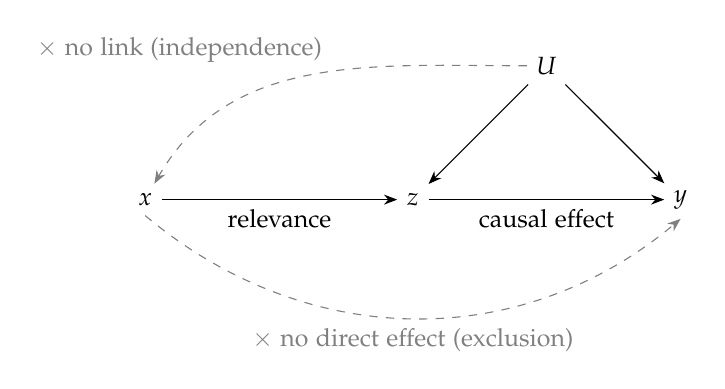
\begin{tikzpicture}[>=Stealth,every node/.style={font=\small}]
\node (x) at (0,0) {$x$};
\node (z) at (3.4,0) {$z$};
\node (y) at (6.8,0) {$y$};
\node (U) at (5.1,1.7) {$U$};
\draw[->] (x) -- node[below]{relevance} (z);
\draw[->] (z) -- node[below]{causal effect} (y);
\draw[->] (U) -- (z);
\draw[->] (U) -- (y);
\draw[->,dashed,gray] (x.south) to[out=-40,in=-140] node[below,pos=0.5]{$\times$ no direct effect (exclusion)} (y.south);
\draw[->,dashed,gray] (U) to[out=180,in=60] node[above left,pos=0.45]{$\times$ no link (independence)} (x);
\end{tikzpicture}
\caption{The IV assumptions. $U$ collects unobservables, such as ability, that affect both the choice of $z$ and the outcome $y$.}\label{fig:iv}
\end{figure}

\paragraph{What can be tested}
Relevance is testable from the first stage. Independence and exclusion cannot be verified from the data; at most some of their implications can be tested, and they must be argued from knowledge of how $x$ is generated.

\paragraph{Where instruments come from}
Good instruments usually come from knowing how treatment was assigned, through ``natural experiments'': lotteries (the Vietnam draft lottery for veteran status, Angrist, 1990); institutional rules (quarter of birth and compulsory-schooling laws, Angrist and Krueger, 1991); geography and costs (distance to college, Card, 1995); randomly assigned decision makers (judge or caseworker leniency; Kling, 2006; Dobbie, Goldin and Yang, 2018); and randomised encouragement, an experiment that changes the incentive to take the treatment without forcing anybody. Lotteries and random assignment deliver independence by design; for geographic and institutional instruments, independence must be argued, and in no case is exclusion guaranteed by design. Each instrument has its own compliers. The cautionary tale is Bound, Jaeger and Baker (1995), who showed that the quarter-of-birth instruments are weak; Section~\ref{sec:weak} returns to that problem.


% ------------------------------------------------------------------
\subsection{GMM: doing it right}\label{sec:gmm}

\begin{asmset}[Chapter 3; Hayashi 3.1--3.5]
\leavevmode
\begin{enumerate}[label=(\roman*)]
\item Linearity: $y_i=z_i'\delta+\varepsilon_i$ with $\dim z_i=L$; $\E[z_i\varepsilon_i]\neq0$ is allowed.
\item $(y_i,z_i,x_i)$ is jointly stationary and ergodic.
\item Orthogonality: $\E[g_i]=\E[x_i\varepsilon_i]=\E\big[x_i(y_i-z_i'\delta)\big]=0$, with $\dim x_i=K$.
\item Rank: $\sxz=\E[x_iz_i']$, a $K\times L$ matrix, has full column rank $L$.
\item $g_i$ is an m.d.s.\ with $S=\E[g_ig_i']$ finite and nonsingular.
\end{enumerate}
\end{asmset}

In vector notation, $z_i$ collects all explanatory variables and $x_i$ everything uncorrelated with $\varepsilon_i$; the exogenous regressors, including the constant, appear in both. Variables in $z_i$ but not in $x_i$ are the endogenous regressors; variables in $x_i$ but not in $z_i$ are the excluded instruments.

\begin{whybox}{GMM}
Many economic theories deliver moment conditions and nothing more: an Euler equation says that a pricing error is unpredictable given current information, an exclusion restriction says that an instrument is uncorrelated with a structural error. Neither specifies the joint distribution of the data, so likelihood methods are unavailable without additional assumptions. GMM takes the moment condition as the primitive and asks how best to exploit it. It also provides a single framework in which OLS ($x=z$), IV ($K=L$), 2SLS and efficient GMM are special cases distinguished only by the instrument list and the weighting matrix.
\end{whybox}

\begin{whybox}{the rank condition is identification}
The orthogonality conditions are $K$ linear equations in $L$ unknowns,
\[
\sxz\,\delta=\sigma_{xy},\qquad\sigma_{xy}=\E[x_iy_i].
\]
A solution exists because the model holds; it is unique if and only if $\sxz$ has full column rank, which requires the order condition $K\geq L$. The order condition has three equivalent readings: at least as many instruments as regressors, at least as many orthogonality conditions as parameters, and at least as many excluded exogenous variables as endogenous regressors. In the supply-and-demand example the rank condition is that the excluded cost shifters actually move the price. Identification is a property of the population and logically prior to estimation: no amount of data rescues a rank-deficient $\sxz$, and a \emph{nearly} rank-deficient one is the weak-instrument problem of Section~\ref{sec:weak}. Because the moments are linear in $\delta$, local and global identification coincide here; in nonlinear GMM they need not.
\end{whybox}

\paragraph{Just identification ($K=L$)}
Then $\delta=\sxz^{-1}\sigma_{xy}$, estimated by
\[
\dhat_{IV}=\Big(\frac1n\sum_{i=1}^nx_iz_i'\Big)^{-1}\frac1n\sum_{i=1}^nx_iy_i=\Sxz^{-1}s_{xy}=\delta+\Sxz^{-1}\,\frac1n\sum_{i=1}^nx_i\varepsilon_i .
\]
Exactly as in Theorem~\ref{thm:ols_asy}, $\dhat_{IV}\cas\delta$ and
\[
\sqrt n(\dhat_{IV}-\delta)=\Sxz^{-1}\,\frac1{\sqrt n}\sum_{i=1}^nx_i\varepsilon_i\;\cd\;\N\big(0,\;\sxz^{-1}S\,\sxz'^{-1}\big).
\]
OLS is the special case $x_i=z_i$: it is the method-of-moments estimator for the moment conditions $\E[z_i\varepsilon_i]=0$. In the just-identified case IV coincides with \emph{indirect least squares}, the ratio of reduced-form to first-stage coefficients, and its residuals are exactly orthogonal to every instrument.

\paragraph{Over-identification ($K>L$)}
The sample moment
\[
g_n(\tilde\delta)=\frac1n\sum_{i=1}^nx_i(y_i-z_i'\tilde\delta)=s_{xy}-\Sxz\tilde\delta
\]
consists of $K$ equations in $L$ unknowns and generically cannot be set to zero, even though the population system $\sxz\delta=\sigma_{xy}$ has an exact solution. The reason is instructive. That the population system is solvable is an \emph{equality} restriction on $(\sxz,\sigma_{xy})$, namely that $\sigma_{xy}$ lies in the column space of $\sxz$, and equality restrictions do not survive sampling noise. Full column rank is an \emph{inequality} restriction, and $\Sxz$ inherits it with probability approaching one. GMM therefore makes the sample moments as close to zero as possible in a chosen metric:
\[
\dhat(\hat W)=\arg\min_{\tilde\delta}\;J(\tilde\delta,\hat W),\qquad J(\tilde\delta,\hat W)=n\,g_n(\tilde\delta)'\,\hat W\,g_n(\tilde\delta),
\]
with $\hat W$ symmetric positive definite and $\hat W\cp W$, also symmetric positive definite. The first-order condition gives
\begin{equation}\label{eq:gmm}
\dhat(\hat W)=\big(\Sxz'\hat W\Sxz\big)^{-1}\Sxz'\hat W\,s_{xy}=\delta+\big(\Sxz'\hat W\Sxz\big)^{-1}\Sxz'\hat W\,\frac1n\sum_{i=1}^nx_i\varepsilon_i .
\end{equation}
Rescaling $\hat W$ by a positive constant leaves the estimator unchanged, and when $K=L$ the weight cancels and $\dhat(\hat W)=\dhat_{IV}$. The first-order condition $\Sxz'\hat Wg_n(\dhat)=0$ sets only $L$ linear combinations of the $K$ sample moments to zero, not the moments themselves; the $K-L$ leftover directions are what the overidentification test of this section examines.

\begin{whybox}{a weighting matrix}
With more equations than unknowns, the sample moments contradict one another, and the estimator must decide which violations to tolerate. $\hat W$ encodes that trade-off: it states how costly a deviation in each direction of moment space is. In the population all $K$ conditions hold simultaneously, so every positive definite $W$ yields a consistent estimator; the choice affects only precision. With exact identification there is nothing to trade off, which is why $W$ then drops out. Note the difference from weighted least squares: WLS weights \emph{observations}, GMM weights \emph{sample moments}, which are averages over all observations.
\end{whybox}

Consistency follows as before: $\dhat(\hat W)\cp\delta$. For the distribution, \eqref{eq:gmm} and Slutsky's lemma give
\[
\sqrt n\big(\dhat(\hat W)-\delta\big)=\big(\Sxz'\hat W\Sxz\big)^{-1}\Sxz'\hat W\,\frac1{\sqrt n}\sum_{i=1}^nx_i\varepsilon_i\;\cd\;\big(\sxz'W\sxz\big)^{-1}\sxz'W\cdot\N(0,S),
\]
that is,
\begin{equation}\label{eq:gmm_avar}
\sqrt n\big(\dhat(\hat W)-\delta\big)\cd\N\Big(0,\;\big(\sxz'W\sxz\big)^{-1}\sxz'WSW\sxz\big(\sxz'W\sxz\big)^{-1}\Big).
\end{equation}
This is the sandwich of Section~\ref{sec:ols_asy} once more: the bread $(\sxz'W\sxz)^{-1}\sxz'W$ translates noise in the moments into noise in the estimate, and the meat $S$ is the variance of the moments. Every estimator in the remainder of these notes is a GMM estimator for some choice of $\hat W$.

\begin{theorem}[Efficient GMM]
The asymptotic variance in \eqref{eq:gmm_avar} is minimised, in the positive-semidefinite order, by $W=S^{-1}$, where it equals $\big(\sxz'S^{-1}\sxz\big)^{-1}$.
\end{theorem}

\begin{proof}
Let $A=(\sxz'W\sxz)^{-1}\sxz'W$ and $B=(\sxz'S^{-1}\sxz)^{-1}\sxz'S^{-1}$, so the two variances are $ASA'$ and $BSB'$. Both satisfy $A\sxz=B\sxz=I_L$. Hence
\[
BSA'=(\sxz'S^{-1}\sxz)^{-1}\sxz'A'=(\sxz'S^{-1}\sxz)^{-1}=BSB',
\]
and therefore $ASA'-BSB'=(A-B)\,S\,(A-B)'\succeq0$.
\end{proof}

\begin{whybox}{efficient GMM is GLS in moment space}
Read $s_{xy}=\Sxz\delta+\bar g_n$, with $\bar g_n=n^{-1}\sum_ix_i\varepsilon_i$, as a ``regression'' of $K$ sample moments on the $K\times L$ matrix $\Sxz$, with an ``error'' whose variance is approximately $S/n$. Weighting by $S^{-1}$ is exactly GLS for this system: moment conditions that are estimated noisily are downweighted, and correlated moment conditions, which partly duplicate one another's information, are not double-counted. The proof above is the Gauss--Markov argument written in a new coordinate system. Two refinements sharpen the reading. Efficiency is relative to the moment conditions used: adding valid instruments can only lower $(\sxz'S^{-1}\sxz)^{-1}$, and with $\E[\varepsilon_i\mid x_i]=0$ the best possible instruments would be the conditional expectation of $z_i$ given $x_i$, scaled by the inverse conditional variance, which is GLS in yet another guise (Hansen, 2022, \S13.27). And by Section~\ref{sec:pitman}, efficiency translates directly into local power of tests: efficient GMM maximises the power of Wald tests against local alternatives.
\end{whybox}

In practice, \emph{two-step GMM} first computes $\dhat(\hat W_1)$ for some convenient $\hat W_1$, usually the 2SLS weight $\Sxx^{-1}$, then forms
\[
\hat S=\frac1n\sum_{i=1}^n\big(y_i-z_i'\dhat(\hat W_1)\big)^2x_ix_i',
\]
and finally computes $\dhat(\hat S^{-1})$. The sole purpose of the first step is a consistent estimate of $S$. The estimator satisfies
\[
\sqrt n\big(\dhat(\hat S^{-1})-\delta\big)\cd\N\big(0,\;(\sxz'S^{-1}\sxz)^{-1}\big),\qquad\widehat\Avar=\big(\Sxz'\hat S^{-1}\Sxz\big)^{-1}.
\]
A third step, recomputing $\hat S$ from second-step residuals, yields no asymptotic gain, since any consistent $\hat S$ delivers the same limit; iterating to convergence removes the dependence on $\hat W_1$ in finite samples. With time-series dependence or clustering, $S$ is replaced by the appropriate long-run or cluster-level variance, and nothing else changes.

\begin{whybox}{efficiency on paper is not always efficiency in samples}
$\hat S$ is an average of fourth moments, $e_i^2x_ix_i'$, which are estimated much less precisely than the second moments in $\Sxz$. Monte Carlo evidence (the 1996 \emph{Journal of Business \& Economic Statistics} symposium on GMM, summarised in Hayashi, 2000, \S3.5) finds that efficient two-step GMM can have larger finite-sample bias than simpler weightings and that its Wald tests over-reject, especially with many moment conditions. The asymptotic ranking is a ranking of limits; how quickly the limits become relevant depends on how hard $S$ is to estimate. This tension between asymptotic efficiency and finite-sample reliability returns with weak and many instruments in Section~\ref{sec:weak} and motivates the continuously updated estimator of Section~\ref{sec:cue}.
\end{whybox}

\paragraph{Testing overidentifying restrictions}

\begin{theorem}[Hansen's $J$-test]
Under the Chapter~3 assumptions, if all instruments are valid,
\[
J\big(\dhat(\hat S^{-1}),\hat S^{-1}\big)\cd\chi^2(K-L).
\]
\end{theorem}

\begin{proof}
Write $\dhat=\dhat(\hat S^{-1})$. Then $g_n(\dhat)=g_n(\delta)-\Sxz(\dhat-\delta)$, and
\[
\sqrt n(\dhat-\delta)=(\sxz'S^{-1}\sxz)^{-1}\sxz'S^{-1}\sqrt n\,g_n(\delta)+\op(1).
\]
Let $F=S^{-1/2}\sxz$ and $u_n=S^{-1/2}\sqrt n\,g_n(\delta)\cd\N(0,I_K)$. Substituting,
\[
S^{-1/2}\sqrt n\,g_n(\dhat)=\big[I_K-F(F'F)^{-1}F'\big]u_n+\op(1)=M_Fu_n+\op(1).
\]
$M_F$ is symmetric and idempotent of rank $K-L$, so $J=u_n'M_Fu_n+\op(1)\cd\chi^2(K-L)$.
\end{proof}

\begin{whybox}{$K-L$ degrees of freedom, and what $J$ can and cannot detect}
Evaluated at the true $\delta$, $J(\delta,\hat S^{-1})=n\,\bar g_n'\hat S^{-1}\bar g_n$ would be $\chi^2(K)$. Estimating $\delta$ uses up $L$ directions of the $K$-dimensional moment space, because the estimator forces the moments to zero along the columns of $F$; only the orthogonal $(K-L)$-dimensional residual remains free to reveal a violation. The loss of degrees of freedom is the same phenomenon as dividing $e'e$ by $n-K$ in Chapter~1. With $K=L$ the minimised criterion is identically zero and there is nothing to test.

The test has three important limitations (Hayashi, 2000, \S3.6). First, it is a test of \emph{all} maintained assumptions, not only of instrument validity, and a large $J$ indicates invalid instruments only if the other assumptions are trusted. Second, it is not consistent against every failure of orthogonality: a violation $\E[x_i\varepsilon_i]=c$ with $c$ in the column space of $\sxz$ can be absorbed by moving $\delta$ and leaves $J$ bounded. A violation proportional to the instruments' covariances with the regressors, $c=\sxz d$, is of this kind: it shifts every just-identified IV estimand by the same $d$, so the instruments still agree with one another and $J$ has nothing to detect. Third, $J$ over-rejects in small samples. There is also a substantive reading. With two excluded instruments for one endogenous regressor, each instrument alone identifies $\delta$, and the overidentifying restriction says that the two just-identified IV estimands coincide. In Card's data, IV with public-college proximity alone gives about $0.16$ and with private-college proximity alone about $0.27$, and the test does not reject (Hansen, 2022, \S12.31). With heterogeneous effects, valid instruments identify different LATEs, so a rejection need not mean that any instrument is invalid. Because no overidentified model is literally true, it is sensible to use small significance levels.
\end{whybox}

% ------------------------------------------------------------------
\subsection{2SLS as efficient GMM under homoskedasticity}\label{sec:2sls}

Suppose $\E[\varepsilon_i^2\mid x_i]=\sigma^2$; note that the conditioning is on the instruments. Then $S=\E\big[\E(\varepsilon_i^2\mid x_i)x_ix_i'\big]=\sigma^2\sxx$, fourth moments are no longer needed, and the first step of two-step GMM becomes unnecessary. Using $\hat S=\sigma^2\Sxx$, in which the scalar $\sigma^2$ cancels,
\begin{align*}
\dhat(\hat S^{-1})&=\big[Z'X(X'X)^{-1}X'Z\big]^{-1}Z'X(X'X)^{-1}X'y\\
&=(Z'P_XZ)^{-1}Z'P_Xy=(\hat Z'\hat Z)^{-1}\hat Z'y,\qquad\hat Z=P_XZ,
\end{align*}
where the last step uses $P_X=P_X'P_X$. 2SLS is therefore efficient GMM under conditional homoskedasticity and is algebraically OLS of $y$ on the first-stage fitted values, with
\[
\Avar(\dhat_{2SLS})=\sigma^2\big(\sxz'\sxx^{-1}\sxz\big)^{-1}.
\]
Under heteroskedasticity 2SLS remains consistent and asymptotically normal, but it is no longer efficient, and its standard errors must use the sandwich \eqref{eq:gmm_avar} with $W=\sxx^{-1}$. Heteroskedasticity is no less likely in IV than in OLS. The matrix $\hat Z=P_XZ$ is also the optimal set of $L$ linear combinations of the $K$ instruments under homoskedasticity: 2SLS reduces an over-identified problem to a just-identified one by using the best linear predictors of the regressors as instruments. Under homoskedasticity the $J$-statistic becomes Sargan's statistic,
\[
J=\frac{\hat\varepsilon'P_X\hat\varepsilon}{\hat\varepsilon'\hat\varepsilon/n}=n\,R^2_{uc},\qquad\hat\varepsilon=y-Z\dhat_{2SLS},
\]
where $R^2_{uc}$ is the uncentred $R^2$ from regressing the 2SLS residuals on all instruments: the test asks whether the instruments can still explain the structural residuals. This form is valid only under homoskedasticity.

The standard errors printed by a literal second-stage OLS regression are wrong. They estimate $\sigma^2$ from $y-\hat Z\dhat$ rather than from $y-Z\dhat$, and the former contains the extra term $(Z-\hat Z)\dhat=\hat v\dhat$, which changes, and typically inflates, the estimated residual variance. For the same reason, second-stage $t$ and $F$ statistics are not valid even in large samples. Use the IV command. For the same reason again, there is no meaningful $R^2$ for 2SLS: its residual sum of squares does not split into explained and unexplained parts.

\begin{example}[Simulated returns to schooling]
The slides simulate $n=500$ observations with
\[
ed=\nu+z_1+z_2/2+ability,\qquad exper=\nu'+z_2,\qquad y=1+ed+exper+ability+u,
\]
all primitive variables standard normal. OLS that controls for ability gives $1.030$ for the coefficient on $ed$, and OLS that omits it gives $1.380$; the population value of the latter is $1+1/3.125=1.32$, the ability bias being $\Cov(ed,ability\mid exper)/\V(ed\mid exper)$. The first stage has $F=122.8$ for $(z_1,z_2)$, and the coefficient on $exper$ in the first stage is essentially zero ($0.006$), as it should be once $z_2$ is controlled for. 2SLS gives $1.028$ with robust standard error $0.064$; the manual second stage reproduces the coefficient but reports a standard error of $0.114$ and a root MSE of $2.53$ instead of $1.45$. LIML gives $1.027$, two-step GMM $1.028$, and the overidentification test has $p=0.448$.
\end{example}

\begin{whybox}{IV is less precise than OLS, and by how much}
The first reading of 2SLS above makes the cost exact. Under homoskedasticity, $\Avar(\dhat_{2SLS})=\sigma^2\E[\tilde z_i\tilde z_i']^{-1}$ with $\tilde z_i=\Gamma'x_i$, which is the OLS formula with the regressor replaced by its instrument-driven part. Since $z_i=\tilde z_i+v_i$ with $\tilde z_i\perp v_i$,
\[
\E[z_iz_i']-\E[\tilde z_i\tilde z_i']=\E[v_iv_i']\succeq0 .
\]
IV discards the first-stage residual $v_i$, the variation in $z$ that may be contaminated, and pays for consistency with exactly that information. In the just-identified, scalar case the variance ratio relative to an (infeasible) exogenous OLS regression is $1/\rho_{zx}^2$, the inverse squared correlation between regressor and instrument. Instrument strength does not affect consistency, as long as the correlation is not zero, but it governs precision, and as the correlation approaches zero the price becomes prohibitive; Section~\ref{sec:weak} shows that the normal approximation itself then breaks down.
\end{whybox}

% ------------------------------------------------------------------
\subsection{LIML, k-class estimators, and the Anderson--Rubin idea}\label{sec:liml}

Partition the structural equation and the first stage as
\[
y_i=x_{1i}'\delta_1+z_{2i}'\delta_2+\varepsilon_i,\qquad z_{2i}'=x_{1i}'\Pi_1+x_{2i}'\Pi_2+V_i,
\]
with $\E[x_{1i}\varepsilon_i]=\E[x_{2i}\varepsilon_i]=0$ and $\E[x_{1i}V_i]=\E[x_{2i}V_i]=0$. Here $x_{1i}=z_{1i}$ are the included exogenous variables, $z_{2i}$ the endogenous regressors and $x_{2i}$ the excluded instruments; the first stage is a projection and entails no loss of generality. Substituting it gives
\[
y_i=x_{1i}'(\delta_1+\Pi_1\delta_2)+x_{2i}'\Pi_2\delta_2+(\varepsilon_i+V_i\delta_2).
\]
2SLS estimates $(\Pi_1,\Pi_2)$ first and then $(\delta_1,\delta_2)$. The limited-information maximum likelihood (LIML) estimator is the MLE that assumes $(\varepsilon_i,V_i)$ jointly normal and models only the equation of interest and the first stage of its endogenous regressors, not the rest of the system. Its logic is best seen by trying a candidate value $g_2$:
\[
y_i-z_{2i}'g_2=x_{1i}'\big(\delta_1+\Pi_1(\delta_2-g_2)\big)+x_{2i}'\Pi_2(\delta_2-g_2)+V_i(\delta_2-g_2)+\varepsilon_i .
\]
The excluded instruments drop out exactly when $g_2=\delta_2$. One can show that LIML for $\delta_2$ minimises over $g_2$ the $F$-statistic for $\alpha_2=0$ in the regression
\[
y_i-z_{2i}'g_2=x_{1i}'\alpha_1+x_{2i}'\alpha_2+\text{error}_i .
\]
Evaluated at a hypothesised value $\delta_2^0$, this $F$-statistic is the \emph{Anderson--Rubin test}. Under $H_0\colon\delta_2=\delta_2^0$ the regression is $y_i-z_{2i}'\delta_2^0=x_{1i}'\delta_1+\varepsilon_i$, so the excluded instruments have zero coefficients whatever the size of $\Pi_2$, and the null distribution of the test does not depend on the strength of the instruments. What that distribution is depends on the error structure, exactly as for any regression $F$-test. With normal, homoskedastic errors and conditioning on the instruments, the statistic is exactly $F(K_2,\,n-K)$, where $K_2=\dim x_{2i}$; with homoskedastic but non-normal errors, $K_2$ times it is asymptotically $\chi^2_{K_2}$; under heteroskedasticity, clustering or serial correlation, one uses the corresponding robust Wald statistic for $\alpha_2=0$, which is asymptotically $\chi^2_{K_2}$. In every case, validity does not require strong instruments. A rejection, however, can reflect either $\delta_2\neq\delta_2^0$ or a failure of the exclusion restrictions, because the test checks both at once.

With $M_X=I-X(X'X)^{-1}X'$ and $M_1=I-X_1(X_1'X_1)^{-1}X_1'$, the $k$-class estimators are
\[
\begin{pmatrix}\dhat_1(k)\\[2pt]\dhat_2(k)\end{pmatrix}=\begin{pmatrix}X_1'X_1&X_1'Z_2\\[2pt]Z_2'X_1&Z_2'(I-kM_X)Z_2\end{pmatrix}^{-1}\begin{pmatrix}X_1'y\\[2pt]Z_2'(I-kM_X)y\end{pmatrix}.
\]
OLS corresponds to $k=0$, 2SLS to $k=1$, and LIML to $k=\hat\kappa$, the smallest eigenvalue of
\[
(Y'M_XY)^{-1/2}\,Y'M_1Y\,(Y'M_XY)^{-1/2},\qquad Y=\big[y\;\; Z_2\big].
\]
All $k$-class estimators with $\sqrt n(k-1)\cp0$ share the same asymptotic distribution, so LIML and 2SLS are first-order equivalent (Davidson and MacKinnon).

\begin{whybox}{the $k$-class is a single dial, and why LIML is often preferred}
The parameter $k$ measures how much of the endogenous variation in $Z_2$ is removed: $Z_2'(I-kM_X)$ subtracts $k$ times the part of $Z_2$ that the instruments do not explain. OLS removes none of it, 2SLS removes all of it. The eigenvalue $\hat\kappa$ is the minimised \emph{least variance ratio}, the variance of the implied structural residual after partialling out only the included exogenous variables, relative to its variance after partialling out all instruments; it satisfies $\hat\kappa\geq1$, with equality when the equation is just identified. LIML therefore moves \emph{further} from OLS than 2SLS does, which is the direction in which the finite-sample bias of 2SLS needs correcting, and in the just-identified case LIML $=$ 2SLS $=$ IV.

First-order equivalence hides finite-sample differences. With many instruments the 2SLS first stage over-fits: $\hat Z=P_XZ$ absorbs part of the endogenous noise $V$ and drifts toward $Z$, pulling 2SLS toward OLS, and LIML does not suffer from this to the same extent. Under normal errors and fixed instruments, 2SLS has finite moments only up to the order of overidentification, so the just-identified IV estimator has no mean (Kinal, 1980), while LIML has no finite moments at all; yet in simulations LIML approaches its normal limit faster and is less biased, at the price of thicker tails. LIML is also invariant to how the structural equation is normalised (which variable is placed on the left-hand side), whereas 2SLS is not. Section~\ref{sec:cue} shows that LIML is a continuously updated GMM estimator, which explains several of these properties.
\end{whybox}

% ------------------------------------------------------------------
\subsection{Weak instruments}\label{sec:weak}

Consider the simple model
\[
y=Z\gamma+u,\qquad Z=X\pi+v,
\]
with scalar $\gamma$ and $K$ instruments $X$ independent of $(u,v)$. Then
\[
\hat\gamma_{2SLS}=\frac{Z'X(X'X)^{-1}X'y}{Z'X(X'X)^{-1}X'Z}=\gamma+\frac{Z'X(X'X)^{-1}X'u}{Z'X(X'X)^{-1}X'Z}.
\]
Let $Q=X'X/n$. Approximately, $X'u/\sqrt n\sim\N(0,\sigma_u^2Q)$ and $X'v/\sqrt n\sim\N(0,\sigma_v^2Q)$, exactly so if $(u,v)$ is normal. Write $X'u/\sqrt n=\sigma_uQ^{1/2}z_u$ and $X'v/\sqrt n=\sigma_vQ^{1/2}z_v$, where $z_u$ and $z_v$ are standard normal $K$-vectors correlated with each other. Since $Z'X/\sqrt n=\sqrt n\,\pi'Q+v'X/\sqrt n$, define the vector
\[
\lambda=\frac{\sqrt n\,Q^{1/2}\pi}{\sigma_v}.
\]
Then
\begin{equation}\label{eq:weak}
\hat\gamma_{2SLS}-\gamma\;\approx\;\frac{\sigma_u}{\sigma_v}\cdot\frac{(\lambda+z_v)'z_u}{(\lambda+z_v)'(\lambda+z_v)} .
\end{equation}

\begin{whybox}{the concentration parameter governs everything}
Equation~\eqref{eq:weak} depends on the first-stage coefficients $\pi$ only through $\mu^2=\lambda'\lambda=n\pi'Q\pi/\sigma_v^2$, the \emph{concentration parameter}, which is the signal-to-noise ratio of the first stage. When $\mu^2$ is large relative to the noise $z_v$, the expression is approximately $(\sigma_u/\sigma_v)\lambda'z_u/\mu^2$, a normal variable with variance $\sigma_u^2/(\sigma_v^2\mu^2)$, and standard asymptotics apply. When $\mu^2$ is small, the ratio is dominated by $z_v'z_u/z_v'z_v$, whose centre is $\sigma_{uv}/\sigma_v^2$, which is precisely the bias of OLS. Weak instruments therefore pull 2SLS toward OLS and make its distribution non-normal; heuristically, the bias relative to OLS is about $K/(K+\mu^2)$. Because the first-stage $F$-statistic satisfies $\E[F]\approx1+\mu^2/K$, the first-stage $F$ is a direct read-out of $\mu^2/K$. LIML suffers from weak instruments as well, though less.

The extreme case $\pi=0$ is instructive. The IV estimator is then inconsistent and remains random in the limit, centred at the OLS limit; in the just-identified case the limit is a Cauchy-type ratio of normals with no finite mean. Worse, when the endogeneity is strong the conventional standard error can be small, so that the $t$-statistic is large: an estimate that carries no information about $\gamma$ is reported as precise (Hansen, 2022, \S12.35).
\end{whybox}

\begin{whybox}{standard asymptotics misleads here, and the fix}
With $\pi\neq0$ fixed, $\mu^2=n\pi'Q\pi/\sigma_v^2\to\infty$ as $n\to\infty$, so conventional asymptotics always ends up in the strong-instrument regime and cannot describe a sample in which $\mu^2$ is moderate. Staiger and Stock (1997) instead let $\pi=C/\sqrt n$, which holds $\lambda$, and therefore $\mu^2$, fixed as $n$ grows. The device is not meant literally; it balances first-stage signal and noise so that the limit retains the feature of the finite-sample problem that matters. The limit is then \eqref{eq:weak} itself, non-normal and centred between $\gamma$ and the OLS limit. The same move, letting the number of instruments grow with $n$, captures the many-instruments problem. In the framework of Bekker (1994), the number of instruments grows in proportion to $n$ while the instruments' aggregate explanatory power for $z$ stays bounded away from zero, so that $\mu^2$ also grows in proportion to $n$. There the 2SLS limit lies strictly between $\gamma$ and the OLS limit and approaches the latter as the ratio of instruments to observations rises, because the first stage fits noise, whereas LIML remains consistent if the errors are homoskedastic. The LIML result needs both qualifications: under heteroskedasticity LIML is in general inconsistent in this framework, and if identification is weak in the sense that $\mu^2$ stays bounded, no estimator is consistent. It is the asymptotic counterpart of the observation that adding weak instruments raises $K$ faster than $\mu^2$. This methodological lesson, choosing the asymptotic experiment to mimic the difficulty at hand, reappears with Pitman drift in Section~\ref{sec:pitman}.
\end{whybox}

\paragraph{Rules of thumb}
In the first stage of 2SLS, regress $z_i$ on $(1,x_{i1},\dots,x_{im},w_{i1},\dots,w_{ir})$, and worry if the $F$-statistic on the excluded instruments is below 10 (Staiger and Stock, 1997). The threshold is not a test that the instruments are relevant, that is, of $\mu^2=0$. It comes from asking how large $\mu^2$ must be for the bias or size distortion of 2SLS to be tolerable and then testing that value, which is why it is far above the conventional critical value; with one instrument it amounts to requiring a first-stage $t$-statistic of roughly 3 rather than $1.96$ (Stock and Yogo, 2005; Hansen, 2022, \S12.38). Even so, the rule is too optimistic for $t$-based inference. With one instrument, the usual 5\% $t$-test has correct size only if $F>104.7$; otherwise one should use adjusted critical values or the Anderson--Rubin test (Lee, McCrary, Moreira and Porter, 2022). In David Lee's words, researchers who used 10 as the threshold and reported $\pm1.96$ intervals ``really had an 88 percent confidence interval''. In Card's data with a single instrument, the first-stage $F$ is about 18, comfortably above 10, yet a conservative calculation that allows for the sampling error in $F$ as an estimate of $\mu^2$ guarantees the conventional 95\% interval only about 80\% coverage (Hansen, 2022, \S12.40). With 180 quarter-of-birth interactions in Angrist and Krueger's data, the first-stage $F$ falls to about $2.4$, and the smaller standard errors that the many instruments produce are a symptom of unreliability, not of precision (Hansen, 2022, \S12.38--12.40).

\paragraph{Weak and slightly invalid instruments}
In $y_i=\beta_0+z_i\beta_1+\varepsilon_i$ with instrument $x_i$ and a constant,
\[
\hat\beta_1=\beta_1+\frac{\frac1n\sum_i(\varepsilon_i-\bar\varepsilon)(x_i-\bar x)}{\frac1n\sum_i(z_i-\bar z)(x_i-\bar x)}\;\cp\;\beta_1+\frac{\Cov(\varepsilon_i,x_i)}{\Cov(z_i,x_i)} .
\]
A small violation of exclusion in the numerator is amplified by a small first stage in the denominator. Weak instruments make IV fragile with respect to exactly the assumptions that cannot be tested, which is the strongest reason to seek instruments that are both strong and credible.


% ==================================================================
\section{Loose ends: power, nonlinear hypotheses, and testing in GMM}\label{sec:loose}
% ==================================================================

The previous sections built estimators and their limit distributions. This section returns to testing and asks three questions that the earlier theory leaves open. How should we compare tests when every reasonable test eventually rejects every false null? What changes when the hypothesis is nonlinear in the parameters? And can the ``fit-deterioration'' logic of the Chapter~1 $F$-test be carried over to GMM? The answers lead back to the choice of weighting matrix and, at the end, to a GMM characterisation of LIML.

\subsection{Consistency is not enough: local alternatives}\label{sec:pitman}

Under the Chapter~2 assumptions, $\sqrt n(\bh_j-\beta_j)\cd\N\big(0,\Avar(\bh_j)\big)$. For $H_0\colon\beta_j=\beta_j^0$ the $t$-statistic satisfies
\[
T_j=\frac{\sqrt n\,(\bh_j-\beta_j^0)}{\sqrt{\widehat\Avar(\bh_j)}}\;\cd\;\N(0,1)\quad\text{under }H_0,
\qquad\text{so}\qquad\Pr\big(|T_j|>t_{\alpha/2}\big)\to\alpha .
\]
Under a fixed alternative $\beta_j\neq\beta_j^0$,
\[
T_j=\frac{\sqrt n\,(\bh_j-\beta_j)}{\sqrt{\widehat\Avar(\bh_j)}}+\frac{\sqrt n\,(\beta_j-\beta_j^0)}{\sqrt{\widehat\Avar(\bh_j)}}\;\cd\;\N(0,1)\pm\infty,
\qquad\text{so}\qquad\Pr\big(|T_j|>t_{\alpha/2}\big)\to1 .
\]
The test is consistent. But the statement holds for \emph{every} estimator with a $\sqrt n$ normal limit, efficient or not, and therefore says nothing about how good the test is. Any consistent test eventually rejects a given false null if the sample is large enough.

\begin{whybox}{we let the alternative drift toward the null}
Asymptotics is a device for approximation, not a belief that anything goes to infinity: we have the data we have. The question we care about is whether a test can detect alternatives that are hard to detect \emph{at our sample size}. The trick is to approximate that situation by a sequence in which the null stays fixed while the alternative approaches it at exactly the rate at which estimation noise shrinks,
\[
\beta_j^{(n)}=\beta_j^0+\frac{\gamma}{\sqrt n}\qquad\text{(Pitman drift)}.
\]
In regular $\sqrt n$ problems of the kind studied in these notes (smooth models with asymptotically normal estimators), alternatives at distance $o(n^{-1/2})$ from the null cannot be distinguished from it: the null and alternative distributions of the data merge, and no test has asymptotic power above its size against them. Alternatives at a distance $d_n$ with $\sqrt n\,d_n\to\infty$ are detected with probability approaching one by the $t$- or Wald test built on a $\sqrt n$-consistent, asymptotically normal estimator with a consistent standard error, because the second term of $T_j$ diverges. In nonregular problems, such as superconsistent estimators or parameters on a boundary, the relevant scale differs. Within the regular framework, the rate $n^{-1/2}$ is the only one at which the drift appears in the limit distribution without dominating it, so only on this scale do tests differ and only there does a comparison have content. The drift $\gamma$ has a simple reading: $\mu=\gamma/\sqrt{\Avar(\bh_j)}\approx(\beta_j^{(n)}-\beta_j^0)/SE(\bh_j)$ is the distance between the alternative and the null measured in standard errors. This is the same methodological move as the local-to-zero first stage of Section~\ref{sec:weak}: choose the asymptotic experiment that preserves the feature of the finite-sample problem that matters.
\end{whybox}

Under the drifting sequence (and regularity conditions we do not spell out),
\begin{align*}
T_j&=\frac{\sqrt n\,\big(\bh_j-\beta_j^{(n)}\big)}{\sqrt{\widehat\Avar(\bh_j)}}+\frac{\sqrt n\,\big(\beta_j^{(n)}-\beta_j^0\big)}{\sqrt{\widehat\Avar(\bh_j)}}\\
&\cd\;\N(0,1)+\frac{\gamma}{\sqrt{\Avar(\bh_j)}}=\N(\mu,1),\qquad\mu=\frac{\gamma}{\sqrt{\Avar(\bh_j)}} .
\end{align*}
The local asymptotic power is therefore
\begin{align}
\Pr\big(|T_j|>t_{\alpha/2}\big)&=\Pr\big(T_j-\mu>t_{\alpha/2}-\mu\big)+\Pr\big(T_j-\mu<-t_{\alpha/2}-\mu\big)\notag\\
&\longrightarrow\;\Phi\big(-t_{\alpha/2}+\mu\big)+\Phi\big(-t_{\alpha/2}-\mu\big).\label{eq:power}
\end{align}

\begin{figure}[h]
\centering
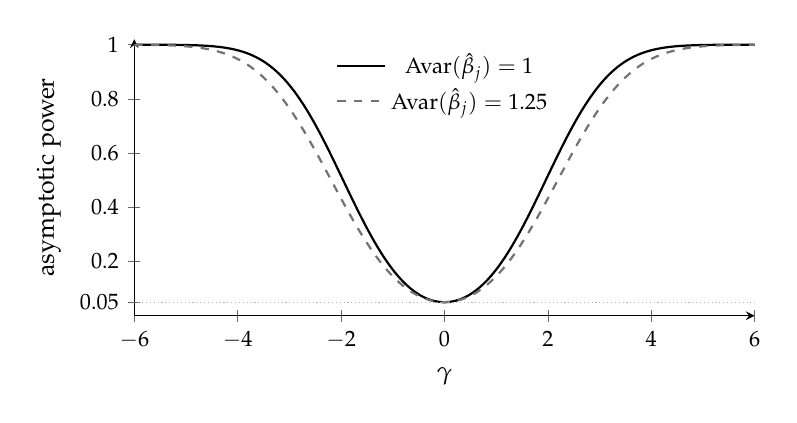
\begin{tikzpicture}
\begin{axis}[
  width=0.78\textwidth,height=0.42\textwidth,
  xmin=-6,xmax=6,ymin=0,ymax=1.02,
  xlabel={$\gamma$},ylabel={asymptotic power},
  xtick={-6,-4,-2,0,2,4,6},ytick={0.05,0.2,0.4,0.6,0.8,1},
  yticklabel style={/pgf/number format/fixed},
  axis lines=left,tick style={black!60},
  every axis label/.style={font=\small},ticklabel style={font=\footnotesize},
  legend style={draw=none,fill=none,font=\footnotesize,at={(0.5,0.99)},anchor=north},
  samples=2,domain=-6:6]
\addplot[black,thick] coordinates {(-6.000,0.99997) (-5.950,0.99997) (-5.900,0.99996) (-5.850,0.99995) (-5.800,0.99994) (-5.750,0.99992) (-5.700,0.99991) (-5.650,0.99989) (-5.600,0.99986) (-5.550,0.99983) (-5.500,0.99980) (-5.450,0.99976) (-5.400,0.99971) (-5.350,0.99965) (-5.300,0.99958) (-5.250,0.99950) (-5.200,0.99940) (-5.150,0.99929) (-5.100,0.99916) (-5.050,0.99900) (-5.000,0.99882) (-4.950,0.99861) (-4.900,0.99836) (-4.850,0.99807) (-4.800,0.99774) (-4.750,0.99736) (-4.700,0.99693) (-4.650,0.99643) (-4.600,0.99586) (-4.550,0.99520) (-4.500,0.99446) (-4.450,0.99361) (-4.400,0.99266) (-4.350,0.99158) (-4.300,0.99036) (-4.250,0.98899) (-4.200,0.98746) (-4.150,0.98574) (-4.100,0.98382) (-4.050,0.98169) (-4.000,0.97933) (-3.950,0.97671) (-3.900,0.97381) (-3.850,0.97062) (-3.800,0.96712) (-3.750,0.96328) (-3.700,0.95907) (-3.650,0.95449) (-3.600,0.94950) (-3.550,0.94409) (-3.500,0.93822) (-3.450,0.93189) (-3.400,0.92507) (-3.350,0.91774) (-3.300,0.90988) (-3.250,0.90148) (-3.200,0.89252) (-3.150,0.88298) (-3.100,0.87286) (-3.050,0.86215) (-3.000,0.85084) (-2.950,0.83892) (-2.900,0.82640) (-2.850,0.81328) (-2.800,0.79956) (-2.750,0.78525) (-2.700,0.77036) (-2.650,0.75492) (-2.600,0.73893) (-2.550,0.72242) (-2.500,0.70542) (-2.450,0.68795) (-2.400,0.67005) (-2.350,0.65175) (-2.300,0.63310) (-2.250,0.61412) (-2.200,0.59486) (-2.150,0.57538) (-2.100,0.55571) (-2.050,0.53590) (-2.000,0.51601) (-1.950,0.49607) (-1.900,0.47615) (-1.850,0.45629) (-1.800,0.43654) (-1.750,0.41695) (-1.700,0.39757) (-1.650,0.37845) (-1.600,0.35962) (-1.550,0.34114) (-1.500,0.32304) (-1.450,0.30536) (-1.400,0.28814) (-1.350,0.27141) (-1.300,0.25520) (-1.250,0.23953) (-1.200,0.22443) (-1.150,0.20992) (-1.100,0.19601) (-1.050,0.18273) (-1.000,0.17008) (-0.950,0.15806) (-0.900,0.14670) (-0.850,0.13598) (-0.800,0.12592) (-0.750,0.11651) (-0.700,0.10775) (-0.650,0.09963) (-0.600,0.09215) (-0.550,0.08531) (-0.500,0.07910) (-0.450,0.07350) (-0.400,0.06852) (-0.350,0.06415) (-0.300,0.06037) (-0.250,0.05719) (-0.200,0.05459) (-0.150,0.05258) (-0.100,0.05115) (-0.050,0.05029) (0.000,0.05000) (0.050,0.05029) (0.100,0.05115) (0.150,0.05258) (0.200,0.05459) (0.250,0.05719) (0.300,0.06037) (0.350,0.06415) (0.400,0.06852) (0.450,0.07350) (0.500,0.07910) (0.550,0.08531) (0.600,0.09215) (0.650,0.09963) (0.700,0.10775) (0.750,0.11651) (0.800,0.12592) (0.850,0.13598) (0.900,0.14670) (0.950,0.15806) (1.000,0.17008) (1.050,0.18273) (1.100,0.19601) (1.150,0.20992) (1.200,0.22443) (1.250,0.23953) (1.300,0.25520) (1.350,0.27141) (1.400,0.28814) (1.450,0.30536) (1.500,0.32304) (1.550,0.34114) (1.600,0.35962) (1.650,0.37845) (1.700,0.39757) (1.750,0.41695) (1.800,0.43654) (1.850,0.45629) (1.900,0.47615) (1.950,0.49607) (2.000,0.51601) (2.050,0.53590) (2.100,0.55571) (2.150,0.57538) (2.200,0.59486) (2.250,0.61412) (2.300,0.63310) (2.350,0.65175) (2.400,0.67005) (2.450,0.68795) (2.500,0.70542) (2.550,0.72242) (2.600,0.73893) (2.650,0.75492) (2.700,0.77036) (2.750,0.78525) (2.800,0.79956) (2.850,0.81328) (2.900,0.82640) (2.950,0.83892) (3.000,0.85084) (3.050,0.86215) (3.100,0.87286) (3.150,0.88298) (3.200,0.89252) (3.250,0.90148) (3.300,0.90988) (3.350,0.91774) (3.400,0.92507) (3.450,0.93189) (3.500,0.93822) (3.550,0.94409) (3.600,0.94950) (3.650,0.95449) (3.700,0.95907) (3.750,0.96328) (3.800,0.96712) (3.850,0.97062) (3.900,0.97381) (3.950,0.97671) (4.000,0.97933) (4.050,0.98169) (4.100,0.98382) (4.150,0.98574) (4.200,0.98746) (4.250,0.98899) (4.300,0.99036) (4.350,0.99158) (4.400,0.99266) (4.450,0.99361) (4.500,0.99446) (4.550,0.99520) (4.600,0.99586) (4.650,0.99643) (4.700,0.99693) (4.750,0.99736) (4.800,0.99774) (4.850,0.99807) (4.900,0.99836) (4.950,0.99861) (5.000,0.99882) (5.050,0.99900) (5.100,0.99916) (5.150,0.99929) (5.200,0.99940) (5.250,0.99950) (5.300,0.99958) (5.350,0.99965) (5.400,0.99971) (5.450,0.99976) (5.500,0.99980) (5.550,0.99983) (5.600,0.99986) (5.650,0.99989) (5.700,0.99991) (5.750,0.99992) (5.800,0.99994) (5.850,0.99995) (5.900,0.99996) (5.950,0.99997) (6.000,0.99997)};
\addlegendentry{$\Avar(\bh_j)=1$}
\addplot[black!55,thick,dashed] coordinates {(-6.000,0.99967) (-5.950,0.99961) (-5.900,0.99955) (-5.850,0.99947) (-5.800,0.99938) (-5.750,0.99927) (-5.700,0.99915) (-5.650,0.99901) (-5.600,0.99885) (-5.550,0.99867) (-5.500,0.99846) (-5.450,0.99822) (-5.400,0.99795) (-5.350,0.99764) (-5.300,0.99729) (-5.250,0.99689) (-5.200,0.99644) (-5.150,0.99593) (-5.100,0.99536) (-5.050,0.99472) (-5.000,0.99400) (-4.950,0.99320) (-4.900,0.99230) (-4.850,0.99130) (-4.800,0.99018) (-4.750,0.98895) (-4.700,0.98758) (-4.650,0.98607) (-4.600,0.98440) (-4.550,0.98256) (-4.500,0.98054) (-4.450,0.97832) (-4.400,0.97590) (-4.350,0.97325) (-4.300,0.97036) (-4.250,0.96721) (-4.200,0.96380) (-4.150,0.96011) (-4.100,0.95611) (-4.050,0.95179) (-4.000,0.94714) (-3.950,0.94214) (-3.900,0.93678) (-3.850,0.93104) (-3.800,0.92490) (-3.750,0.91836) (-3.700,0.91140) (-3.650,0.90400) (-3.600,0.89616) (-3.550,0.88787) (-3.500,0.87911) (-3.450,0.86988) (-3.400,0.86017) (-3.350,0.84998) (-3.300,0.83932) (-3.250,0.82816) (-3.200,0.81653) (-3.150,0.80441) (-3.100,0.79182) (-3.050,0.77877) (-3.000,0.76526) (-2.950,0.75131) (-2.900,0.73692) (-2.850,0.72212) (-2.800,0.70693) (-2.750,0.69137) (-2.700,0.67545) (-2.650,0.65920) (-2.600,0.64266) (-2.550,0.62584) (-2.500,0.60878) (-2.450,0.59151) (-2.400,0.57406) (-2.350,0.55646) (-2.300,0.53875) (-2.250,0.52097) (-2.200,0.50314) (-2.150,0.48532) (-2.100,0.46752) (-2.050,0.44979) (-2.000,0.43216) (-1.950,0.41467) (-1.900,0.39735) (-1.850,0.38023) (-1.800,0.36335) (-1.750,0.34674) (-1.700,0.33042) (-1.650,0.31443) (-1.600,0.29879) (-1.550,0.28353) (-1.500,0.26866) (-1.450,0.25421) (-1.400,0.24020) (-1.350,0.22665) (-1.300,0.21356) (-1.250,0.20096) (-1.200,0.18884) (-1.150,0.17723) (-1.100,0.16613) (-1.050,0.15554) (-1.000,0.14547) (-0.950,0.13592) (-0.900,0.12690) (-0.850,0.11839) (-0.800,0.11040) (-0.750,0.10293) (-0.700,0.09598) (-0.650,0.08953) (-0.600,0.08359) (-0.550,0.07815) (-0.500,0.07321) (-0.450,0.06876) (-0.400,0.06479) (-0.350,0.06130) (-0.300,0.05829) (-0.250,0.05575) (-0.200,0.05367) (-0.150,0.05206) (-0.100,0.05092) (-0.050,0.05023) (0.000,0.05000) (0.050,0.05023) (0.100,0.05092) (0.150,0.05206) (0.200,0.05367) (0.250,0.05575) (0.300,0.05829) (0.350,0.06130) (0.400,0.06479) (0.450,0.06876) (0.500,0.07321) (0.550,0.07815) (0.600,0.08359) (0.650,0.08953) (0.700,0.09598) (0.750,0.10293) (0.800,0.11040) (0.850,0.11839) (0.900,0.12690) (0.950,0.13592) (1.000,0.14547) (1.050,0.15554) (1.100,0.16613) (1.150,0.17723) (1.200,0.18884) (1.250,0.20096) (1.300,0.21356) (1.350,0.22665) (1.400,0.24020) (1.450,0.25421) (1.500,0.26866) (1.550,0.28353) (1.600,0.29879) (1.650,0.31443) (1.700,0.33042) (1.750,0.34674) (1.800,0.36335) (1.850,0.38023) (1.900,0.39735) (1.950,0.41467) (2.000,0.43216) (2.050,0.44979) (2.100,0.46752) (2.150,0.48532) (2.200,0.50314) (2.250,0.52097) (2.300,0.53875) (2.350,0.55646) (2.400,0.57406) (2.450,0.59151) (2.500,0.60878) (2.550,0.62584) (2.600,0.64266) (2.650,0.65920) (2.700,0.67545) (2.750,0.69137) (2.800,0.70693) (2.850,0.72212) (2.900,0.73692) (2.950,0.75131) (3.000,0.76526) (3.050,0.77877) (3.100,0.79182) (3.150,0.80441) (3.200,0.81653) (3.250,0.82816) (3.300,0.83932) (3.350,0.84998) (3.400,0.86017) (3.450,0.86988) (3.500,0.87911) (3.550,0.88787) (3.600,0.89616) (3.650,0.90400) (3.700,0.91140) (3.750,0.91836) (3.800,0.92490) (3.850,0.93104) (3.900,0.93678) (3.950,0.94214) (4.000,0.94714) (4.050,0.95179) (4.100,0.95611) (4.150,0.96011) (4.200,0.96380) (4.250,0.96721) (4.300,0.97036) (4.350,0.97325) (4.400,0.97590) (4.450,0.97832) (4.500,0.98054) (4.550,0.98256) (4.600,0.98440) (4.650,0.98607) (4.700,0.98758) (4.750,0.98895) (4.800,0.99018) (4.850,0.99130) (4.900,0.99230) (4.950,0.99320) (5.000,0.99400) (5.050,0.99472) (5.100,0.99536) (5.150,0.99593) (5.200,0.99644) (5.250,0.99689) (5.300,0.99729) (5.350,0.99764) (5.400,0.99795) (5.450,0.99822) (5.500,0.99846) (5.550,0.99867) (5.600,0.99885) (5.650,0.99901) (5.700,0.99915) (5.750,0.99927) (5.800,0.99938) (5.850,0.99947) (5.900,0.99955) (5.950,0.99961) (6.000,0.99967)};
\addlegendentry{$\Avar(\bh_j)=1.25$}
\addplot[black!30,densely dotted,domain=-6:6] {0.05};
\end{axis}
\end{tikzpicture}
\caption{Local asymptotic power \eqref{eq:power} as a function of the drift $\gamma$, for two estimators with $\Avar(\bh_j)=1$ and $1.25$, at $\alpha=0.05$. Both curves equal the size $0.05$ at $\gamma=0$. This reproduces the figure on the Loose Ends slides from its formula.}\label{fig:power}
\end{figure}

\begin{whybox}{efficiency is power}
Equation \eqref{eq:power} depends on the estimator only through $\mu=\gamma/\sqrt{\Avar(\bh_j)}$, so the test built on the estimator with the smaller asymptotic variance has uniformly higher local power (Figure~\ref{fig:power}). The comparison also has a sample-size reading. Fix an alternative at distance $d$ from the null; then $\gamma=\sqrt n\,d$ and $\mu=d\sqrt{n/\Avar(\bh_j)}$. Two tests have the same power when $n_1/\Avar_1=n_2/\Avar_2$, so an estimator with $\Avar=1.25$ needs 25\% more observations to match the power of one with $\Avar=1$. Every efficiency result of these notes (Gauss--Markov, GLS, efficient GMM) is therefore also a statement about the ability to detect false hypotheses, and the ratio of asymptotic variances is the ratio of sample sizes needed for equal power. The numbers are sobering: an alternative one standard error away from the null ($\mu=1$) is detected by a two-sided 5\% test only about 17\% of the time, and 50\% power requires $\mu\approx1.96$. A ``non-significant'' coefficient is therefore weak evidence that the effect is small unless the standard error is small relative to the effects one cares about.
\end{whybox}

\subsection{Nonlinear hypotheses and the Wald statistic}

Economic restrictions are often nonlinear: a long-run multiplier $\beta_1/(1-\beta_2)$, constant returns in a Cobb--Douglas specification written in levels, a product of a pass-through coefficient and an elasticity. Write the null as
\[
H_0\colon\;a(\beta)=0,\qquad a\colon\R^K\to\R^r,\qquad A(\beta)=\frac{\partial a(\beta)}{\partial\beta'}\ \ (r\times K)\ \text{ of rank }r,
\]
with $a(\cdot)$ continuously differentiable. The delta method, now in the form used on the slides, states that if $x_n\cp\beta$, $\sqrt n(x_n-\beta)\cd z$, and $a(\cdot)$ has continuous first derivatives, then $\sqrt n\big(a(x_n)-a(\beta)\big)\cd A(\beta)z$; in particular, if $\sqrt n(x_n-\beta)\cd\N(0,\Sigma)$, then $\sqrt n\big(a(x_n)-a(\beta)\big)\cd\N\big(0,A(\beta)\Sigma A(\beta)'\big)$. Applied to $\bh$,
\[
\sqrt n\big(a(\bh)-a(\beta)\big)\cd\N\big(0,\;A(\beta)\Avar(\bh)A(\beta)'\big),
\]
and under the null $a(\beta)=0$. Since $A(\bh)\,\widehat\Avar(\bh)\,A(\bh)'\cp A(\beta)\Avar(\bh)A(\beta)'$ by continuity and Slutsky, Lemma~\ref{lem:wald} gives
\begin{equation}\label{eq:nlwald}
W=\big(\sqrt n\,a(\bh)\big)'\Big[A(\bh)\,\widehat\Avar(\bh)\,A(\bh)'\Big]^{-1}\big(\sqrt n\,a(\bh)\big)\;\cd\;\chi^2_r\qquad\text{under }H_0 .
\end{equation}
The rank condition on $A(\beta)$ is what makes the middle matrix invertible: each of the $r$ restrictions must move independently with $\beta$ near the truth.

\paragraph{The Wald statistic is not invariant}
A given hypothesis can usually be written in more than one way. The restrictions
\[
\beta_1\beta_2-1=0,\qquad\beta_1-\frac{1}{\beta_2}=0,\qquad\exp(\beta_1\beta_2-1)+\beta_1\beta_2-2=0
\]
define the same null set, but they yield different values of $W$. Invertible linear rewritings of a linear restriction do not have this defect. If $R'\beta=r$ is rewritten as $AR'\beta=Ar$ with $A$ an invertible square matrix of dimension $\dim(r)$ (not to be confused with the Jacobian $A(\beta)$),
\begin{align*}
W_A&=n\big(AR'\bh-Ar\big)'\Big[AR'\,\widehat\Avar(\bh)\,RA'\Big]^{-1}\big(AR'\bh-Ar\big)\\
&=n\big(R'\bh-r\big)'A'\,(A')^{-1}\Big[R'\,\widehat\Avar(\bh)\,R\Big]^{-1}A^{-1}A\,\big(R'\bh-r\big)=W .
\end{align*}

\begin{whybox}{nonlinear Wald tests depend on how the null is written}
The Wald statistic evaluates the hypothesis at the \emph{unrestricted} estimate and measures the distance of $a(\bh)$ from zero in the metric of its own linearised variance. A nonlinear reparametrisation $\tilde a=h(a)$ with $h(0)=0$ leaves the null set unchanged but alters both the numerator and the linearisation, and the two alterations cancel only to first order at the truth. The statistics are asymptotically equivalent under the null and under local alternatives; in finite samples, and especially when $\bh$ lies far from the null or near a region where $a(\cdot)$ is strongly curved (dividing by a $\beta_2$ close to zero, say), they can differ dramatically. With a linear $a(\cdot)$ the linearisation is exact, which is why the invariance argument above goes through. The magnitudes can be startling. For a ratio $\theta=\beta_1/\beta_2$ with $\beta_2$ small relative to its standard error, the $t$-test based on $\hat\beta_1/\hat\beta_2-\theta_0$ can reject in one tail about half the time and never in the other, at a nominal 5\% level, whereas the equivalent linear form $\hat\beta_1-\theta_0\hat\beta_2$ has essentially exact size (Gregory and Veall, 1985; Hansen, 2022, \S9.17). In practice one should state the restriction in the form in which $a(\bh)$ is closest to linear and its normal approximation most credible, ideally linear, or use a test that does not depend on the parametrisation, which is the subject of the next subsection.
\end{whybox}

\subsection{The likelihood-ratio principle in GMM}\label{sec:gmmlr}

The Chapter~1 $F$-statistic has two faces (Section~\ref{sec:ch1}): a Wald form, which looks only at the unrestricted estimate, and a fit-deterioration form, $e^{*\prime}e^*-e'e$, which compares the restricted and unrestricted criteria. GMM has the same two faces. The efficient estimator minimises the criterion
\begin{gather*}
\dhat(\hat S^{-1})=\arg\min_{\tilde\delta}J(\tilde\delta,\hat S^{-1}),\\
J(\tilde\delta,\hat S^{-1})=n\,g_n(\tilde\delta)'\hat S^{-1}g_n(\tilde\delta)=n\,(s_{xy}-\Sxz\tilde\delta)'\hat S^{-1}(s_{xy}-\Sxz\tilde\delta),
\end{gather*}
with $\hat S$ consistent for $S$. To test $H_0\colon a(\delta)=0$, impose the restriction and see whether it makes a difference. Define the restricted efficient GMM estimator, computed with the \emph{same} $\hat S$,
\[
\bar\delta(\hat S^{-1})=\arg\min_{\tilde\delta}J(\tilde\delta,\hat S^{-1})\quad\text{subject to}\quad a(\tilde\delta)=0,
\]
and the distance statistic
\begin{equation}\label{eq:gmmlr}
LR=J\big(\bar\delta(\hat S^{-1}),\hat S^{-1}\big)-J\big(\dhat(\hat S^{-1}),\hat S^{-1}\big).
\end{equation}
Let $W$ be the Wald statistic \eqref{eq:nlwald} built on $\dhat(\hat S^{-1})$ with $\widehat\Avar=(\Sxz'\hat S^{-1}\Sxz)^{-1}$, and let $A(\delta)=\partial a(\delta)/\partial\delta'$ ($r\times L$) have rank $r$. Under the null, $LR$ and $W$ have the same $\chi^2_r$ limit, $LR-W\cp0$, and if the restriction is linear, $R'\delta-r=0$, then $LR=W$ exactly.

\begin{whybox}{$LR=W$ for linear restrictions}
With linear moments, $J$ is an exact quadratic function of $\tilde\delta$. Expanding around its minimiser, where the first-order condition kills the cross term,
\[
J(\tilde\delta,\hat S^{-1})=J(\dhat,\hat S^{-1})+n\,(\tilde\delta-\dhat)'\big(\Sxz'\hat S^{-1}\Sxz\big)(\tilde\delta-\dhat).
\]
Minimising the second term subject to $R'\tilde\delta=r$ is the restricted least-squares problem of Chapter~1 in the metric $\Sxz'\hat S^{-1}\Sxz$, and the minimised value is
\[
n\,(R'\dhat-r)'\Big[R'\big(\Sxz'\hat S^{-1}\Sxz\big)^{-1}R\Big]^{-1}(R'\dhat-r)=W .
\]
This is the identity $e^{*\prime}e^*-e'e=(R'\bh-r)'[R'(X'X)^{-1}R]^{-1}(R'\bh-r)$ of Chapter~1, with $J$ playing the role of the sum of squared residuals. For nonlinear restrictions the criterion is quadratic only approximately near the truth, so the identity becomes the asymptotic equivalence $LR-W\cp0$.
\end{whybox}

The two principles differ in practice in ways worth remembering.
\begin{itemize}
\item $LR$ is invariant to the way $a(\delta)$ is written, because it depends on the restriction only through the restricted minimum of $J$, i.e.\ through the null set itself. $W$ is not. With a common $\hat S$, moreover, $LR\geq0$ always, because the restricted minimum cannot be below the unrestricted one.
\item $LR$ requires the efficient weight. With an arbitrary $W$, the increase in $J$ is a weighted sum of $\chi^2_1$ variables with unknown weights rather than a $\chi^2_r$, because only $S^{-1}$ makes $J$ a properly standardised quadratic form, exactly as in the derivation of Hansen's $J$-test. The Wald statistic works with any weight, provided $\widehat\Avar$ is the corresponding sandwich.
\item Both criteria must use the same $\hat S$. One may, in principle, use different consistent estimators of $S$ in the two minimisations,
\[
\widetilde{LR}=J\big(\bar\delta(\tilde S^{-1}),\tilde S^{-1}\big)-J\big(\dhat(\hat S^{-1}),\hat S^{-1}\big),
\]
and still have $LR-\widetilde{LR}\cp0$, but $\widetilde{LR}$ can then be negative in small samples. Likewise, if $W$ uses a different consistent estimator of $S$ from the one in $LR$, the exact equality for linear restrictions no longer holds.
\item For nonlinear $a(\delta)$, $LR$ typically requires a numerical constrained optimisation; $W$ requires only the unrestricted estimate.
\end{itemize}
This is the trinity of Section~\ref{sec:ml} once more: Wald looks from the unrestricted estimate, the distance statistic compares the two criteria, and, as there, the comparison of criteria buys invariance at the price of computation. The requirement of efficient weighting is the GMM counterpart of the information-matrix equality that the likelihood-ratio test needs in maximum likelihood: only then is the curvature of the criterion equal to the inverse variance of the estimator, so that a change in the criterion can be read in units of sampling noise.

\subsection{Efficient GMM revisited: two-step and continuously updated}\label{sec:cue}

Recall that $\dhat(\hat W)=\arg\min_{\tilde\delta}n\,g_n(\tilde\delta)'\hat Wg_n(\tilde\delta)$ with $g_n(\tilde\delta)=n^{-1}\sum_ix_i(y_i-z_i'\tilde\delta)$, and that the optimal $\hat W$ is a consistent estimator of $S^{-1}=\E[\varepsilon_i^2x_ix_i']^{-1}$. The two-step estimator makes this feasible by writing
\[
\hat S(d)=\frac1n\sum_{i=1}^n(y_i-z_i'd)^2x_ix_i',\qquad\dhat_{2S}=\arg\min_{\tilde\delta}n\,g_n(\tilde\delta)'\,\hat S\big(\dhat(\hat W_1)\big)^{-1}g_n(\tilde\delta),
\]
so that the weight is evaluated once, at a first-step estimate computed with an arbitrary $\hat W_1$. The \emph{continuously updated estimator} of Hansen, Heaton and Yaron (1996) lets the weight move with the candidate parameter:
\begin{equation}\label{eq:cue}
\dhat_{CUE}=\arg\min_{\tilde\delta}\;n\,g_n(\tilde\delta)'\,\hat S(\tilde\delta)^{-1}g_n(\tilde\delta).
\end{equation}
It needs no ad hoc first-step weighting matrix, and it is invariant to rotations of the moment functions: replacing $g_i(\tilde\delta)$ by $R\,g_i(\tilde\delta)$, or by $R(\tilde\delta)g_i(\tilde\delta)$, with $R$ of full rank $K$, leaves the estimator numerically unchanged, because $g_n\mapsto Rg_n$ and $\hat S\mapsto R\hat SR'$ cancel inside the quadratic form.

\begin{whybox}{update the weight}
Two-step GMM fixes the metric at a preliminary guess and then searches, so the outcome depends on that guess and on how the moments happen to be combined. CUE asks a single, self-consistent question: for each candidate $\tilde\delta$, how large is the moment violation \emph{relative to its own sampling variability at $\tilde\delta$}? That is why it does not depend on a first step or on how the moments are linearly combined. Two-step, iterated and continuously updated GMM are asymptotically equivalent; they differ in finite samples, and the differences are largest when instruments are many or weak. CUE typically has smaller bias but thicker tails, and because $\hat S(\tilde\delta)$ depends on $\tilde\delta$ the criterion is no longer quadratic and must be minimised numerically. Invariance is not a trivial property: two-step GMM is not invariant to parameter-dependent transformations of the moment functions, $g_i\mapsto R(\delta)g_i$ (renormalising an Euler equation, or choosing which variable to put on the left of a structural equation), and with an arbitrary first-step weight not even to a fixed $R$. CUE is invariant to both, which is the property behind LIML's invariance to normalisation, a property 2SLS lacks.
\end{whybox}

In the linear IV model, $g_i(\tilde\delta)=(y_i-z_i'\tilde\delta)x_i$, so
\[
\dhat_{CUE}=\arg\min_{\tilde\delta}\;\Big[\frac1n\sum_{i=1}^n(y_i-z_i'\tilde\delta)x_i\Big]'\Big[\frac1n\sum_{i=1}^n(y_i-z_i'\tilde\delta)^2x_ix_i'\Big]^{-1}\Big[\frac1n\sum_{i=1}^n(y_i-z_i'\tilde\delta)x_i\Big].
\]
Under homoskedasticity $S=\sigma^2\E[x_ix_i']$, which suggests the estimator
\[
\hat S(\tilde\delta)=\Big[\frac1n\sum_{i=1}^n(y_i-z_i'\tilde\delta)^2\Big]\cdot\frac1n\sum_{i=1}^nx_ix_i',
\]
and the continuously updated estimator becomes
\begin{equation}\label{eq:cueliml}
\begin{aligned}
\dhat_{CUE}&=\arg\min_{\tilde\delta}\;\frac{\big[\frac1n\sum_i(y_i-z_i'\tilde\delta)x_i\big]'\big[\frac1n\sum_ix_ix_i'\big]^{-1}\big[\frac1n\sum_i(y_i-z_i'\tilde\delta)x_i\big]}{\frac1n\sum_i(y_i-z_i'\tilde\delta)^2}\\[4pt]
&=\arg\min_{\tilde\delta}\;\frac{u(\tilde\delta)'P_Xu(\tilde\delta)}{u(\tilde\delta)'u(\tilde\delta)},
\end{aligned}
\end{equation}
with $u(\tilde\delta)=y-Z\tilde\delta$. This happens to be the LIML estimator.

\begin{whybox}{the homoskedastic CUE is LIML, and 2SLS is its two-step cousin}
Under homoskedasticity the two-step estimator holds $\sigma^2$ fixed at a first-step value, so it minimises the numerator $u'P_Xu$ alone, and that is 2SLS. CUE divides by $u'u$, re-estimating $\sigma^2$ at every candidate. Since $u'u=u'P_Xu+u'M_Xu$ and $a/(a+b)$ is increasing in $a/b$, minimising $u'P_Xu/u'u$ is the same as minimising $u'P_Xu/u'M_Xu$: the variation in the residual that the instruments explain relative to the variation they leave unexplained. That is the variance-ratio logic of the Anderson--Rubin statistic, through which LIML was characterised in Section~\ref{sec:liml}. The difference between 2SLS and LIML is therefore nothing more than whether the error variance in the GMM weight is updated with the parameter. The ratio is scale-free: it measures the share of the residual variation that the instruments still explain, which is zero in population at the truth whatever the size of the structural error. This offers one way to see why LIML is less exposed than 2SLS to the many-instrument bias toward OLS.
\end{whybox}

% ==================================================================
\section{Synthesis}\label{sec:synth}
% ==================================================================

Table~\ref{tab:synth} collects the estimators of the week as solutions of moment conditions.

\begin{table}[h]
\centering\footnotesize
\setlength{\tabcolsep}{4pt}
\caption{One framework, many estimators}\label{tab:synth}
\begin{tabular}{@{}lllll@{}}
\toprule
Estimator & Moment condition & Weight & Asymptotic variance & Efficient when \\
\midrule
OLS & $\E[x_i(y_i-x_i'\beta)]=0$ & -- & $\sxx^{-1}S\sxx^{-1}$ & $\E[\varepsilon_i^2\mid x_i]=\sigma^2$ \\
GLS & $\E[\sigma_i^{-2}x_i(y_i-x_i'\beta)]=0$ & -- & $\E[\sigma_i^{-2}x_ix_i']^{-1}$ & $\sigma_i^2$ correct \\
IV ($K=L$) & $\E[x_i(y_i-z_i'\delta)]=0$ & -- & $\sxz^{-1}S\sxz'^{-1}$ & always \\
2SLS & same, $K\geq L$ & $\Sxx^{-1}$ & $\sigma^2(\sxz'\sxx^{-1}\sxz)^{-1}$ & $\E[\varepsilon_i^2\mid x_i]=\sigma^2$ \\
GMM & same, $K\geq L$ & $\hat W$ & equation \eqref{eq:gmm_avar} & $W=S^{-1}$ \\
CUE & same, $K\geq L$ & $\hat S(\tilde\delta)^{-1}$ & $(\sxz'S^{-1}\sxz)^{-1}$ & always; $=$ LIML if homosk.\ \\
\bottomrule
\end{tabular}
\end{table}

Three ideas recur throughout the week and organise everything else.

The first is the \emph{analogy principle}. Parameters are defined by population moment conditions; estimators solve their sample analogues. Identification is the uniqueness of the population solution, expressed each time as a rank condition: $\rank X=K$, the invertibility of $\E[x_ix_i']$, the full column rank of $\E[x_iz_i']$. The moment that defines a parameter also defines what the estimator estimates. When OLS seems to ``fail'', it is the moment that is wrong for the question, never the estimator for its moment.

The second is the \emph{sandwich}. Every asymptotic variance has the form $J^{-1}SJ^{-1\prime}$, with $J$ the Jacobian of the moment and $S$ the variance of the score. Homoskedasticity, the information-matrix equality and efficient weighting are three versions of the same event: the meat becoming proportional to the bread, so that the sandwich collapses to a single inverse. Robust, clustered and HAC standard errors are three ways of estimating the meat without modelling it, by averaging over the units that are truly independent.

The third is the \emph{Gauss--Markov template}. OLS under spherical errors, GLS under known heteroskedasticity, and GMM with $W=S^{-1}$ are each optimal because every competitor equals the optimal estimator plus an uncorrelated component. Efficient weighting is always GLS in the appropriate space, and by the local-power argument of Section~\ref{sec:pitman} every efficiency gain is also a gain in the power of tests.

A fourth idea, which the Loose Ends lecture makes explicit, governs testing. Every restriction can be tested in two ways: by asking whether the unrestricted estimate violates it by more than sampling noise allows (Wald), or by asking how much the criterion deteriorates when it is imposed (the $F$-test as a difference of sums of squared residuals, the GMM distance statistic as a difference of $J$'s). For linear restrictions and efficient weighting the two coincide exactly; for nonlinear restrictions only the second is invariant to how the restriction is written. The continuously updated estimator applies the same self-consistency to estimation itself, and under homoskedasticity it reproduces LIML.

Read vertically, the week has a single plot. Chapter~1 identifies the assumptions that make OLS exact and optimal. Chapter~2 shows that consistency and normality require only a population orthogonality condition, a law of large numbers and a central limit theorem; that homoskedasticity matters only for the variance formula; and that the correct variance can be estimated without knowing the heteroskedasticity or the within-cluster dependence. Chapter~3 shows that when orthogonality fails for the regressors, the same machinery runs on orthogonality conditions supplied by instruments. What the resulting estimand means, a weighted average of individual effects with weights given by the instrument's power to move each individual's treatment, and how reliable its inference is, governed by the concentration parameter, depend on the instrument rather than on the estimator.

% ==================================================================
\section*{References}
\addcontentsline{toc}{section}{References}
\markboth{References}{}
% ==================================================================
{\small
\setstretch{1.1}
\begin{description}[leftmargin=1.4em,labelindent=0pt,itemsep=2pt,font=\normalfont]
\item Abadie, A., S.~Athey, G.~W.~Imbens and J.~M.~Wooldridge (2023). When should you adjust standard errors for clustering? \emph{Quarterly Journal of Economics} 138, 1--35.
\item Andrews, I., J.~H.~Stock and L.~Sun (2019). Weak instruments in instrumental variables regression: theory and practice. \emph{Annual Review of Economics} 11, 727--753.
\item Angrist, J.~D. (1990). Lifetime earnings and the Vietnam era draft lottery: evidence from social security administrative records. \emph{American Economic Review} 80, 313--336.
\item Angrist, J.~D.\ and A.~B.~Krueger (1991). Does compulsory school attendance affect schooling and earnings? \emph{Quarterly Journal of Economics} 106, 979--1014.
\item Angrist, J.~D.\ and G.~W.~Imbens (1995). Two-stage least squares estimation of average causal effects in models with variable treatment intensity. \emph{Journal of the American Statistical Association} 90, 431--442.
\item Angrist, J.~D., G.~W.~Imbens and D.~B.~Rubin (1996). Identification of causal effects using instrumental variables. \emph{Journal of the American Statistical Association} 91, 444--455.
\item Angrist, J.~D.\ and J.-S.~Pischke (2009). \emph{Mostly Harmless Econometrics}. Princeton University Press.
\item Bekker, P.~A. (1994). Alternative approximations to the distributions of instrumental variable estimators. \emph{Econometrica} 62, 657--681.
\item Belloni, A., V.~Chernozhukov and C.~Hansen (2014). Inference on treatment effects after selection among high-dimensional controls. \emph{Review of Economic Studies} 81, 608--650.
\item Berndt, E.~R.\ and N.~E.~Savin (1977). Conflict among criteria for testing hypotheses in the multivariate linear regression model. \emph{Econometrica} 45, 1263--1277.
\item Blandhol, C., J.~Bonney, M.~Mogstad and A.~Torgovitsky (2022). When is TSLS actually LATE? NBER Working Paper 29709.
\item Bound, J., D.~A.~Jaeger and R.~M.~Baker (1995). Problems with instrumental variables estimation when the correlation between the instruments and the endogenous explanatory variable is weak. \emph{Journal of the American Statistical Association} 90, 443--450.
\item Card, D. (1995). Using geographic variation in college proximity to estimate the return to schooling. In L.~Christofides, E.~Grant and R.~Swidinsky (eds.), \emph{Aspects of Labour Market Behaviour}. University of Toronto Press.
\item Card, D. (2001). Estimating the return to schooling: progress on some persistent econometric problems. \emph{Econometrica} 69, 1127--1160.
\item Cameron, A.~C., J.~B.~Gelbach and D.~L.~Miller (2008). Bootstrap-based improvements for inference with clustered errors. \emph{Review of Economics and Statistics} 90, 414--427.
\item Cameron, A.~C., J.~B.~Gelbach and D.~L.~Miller (2011). Robust inference with multiway clustering. \emph{Journal of Business \& Economic Statistics} 29, 238--249.
\item Cameron, A.~C.\ and D.~L.~Miller (2015). A practitioner's guide to cluster-robust inference. \emph{Journal of Human Resources} 50, 317--372.
\item Davidson, R.\ and J.~G.~MacKinnon (1993). \emph{Estimation and Inference in Econometrics}. Oxford University Press.
\item Dobbie, W., J.~Goldin and C.~S.~Yang (2018). The effects of pretrial detention on conviction, future crime, and employment: evidence from randomly assigned judges. \emph{American Economic Review} 108, 201--240.
\item Gregory, A.~W.\ and M.~R.~Veall (1985). Formulating Wald tests of nonlinear restrictions. \emph{Econometrica} 53, 1465--1468.
\item Hansen, B.~E. (2022). \emph{Econometrics}. Princeton University Press.
\item Hansen, L.~P. (1982). Large sample properties of generalized method of moments estimators. \emph{Econometrica} 50, 1029--1054.
\item Hansen, L.~P., J.~Heaton and A.~Yaron (1996). Finite-sample properties of some alternative GMM estimators. \emph{Journal of Business \& Economic Statistics} 14, 262--280.
\item Hayashi, F. (2000). \emph{Econometrics}. Princeton University Press.
\item Hong, Y. (2020). \emph{Foundations of Modern Econometrics: A Unified Approach}. World Scientific. (Chinese edition: \emph{Advanced Econometrics}, Higher Education Press.)
\item Imbens, G.~W.\ and J.~D.~Angrist (1994). Identification and estimation of local average treatment effects. \emph{Econometrica} 62, 467--475.
\item Kinal, T.~W. (1980). The existence of moments of $k$-class estimators. \emph{Econometrica} 48, 241--249.
\item Kling, J.~R. (2006). Incarceration length, employment, and earnings. \emph{American Economic Review} 96, 863--876.
\item Lee, D.~S., J.~McCrary, M.~J.~Moreira and J.~Porter (2022). Valid $t$-ratio inference for IV. \emph{American Economic Review} 112, 3260--3290.
\item MacKinnon, J.~G.\ and H.~White (1985). Some heteroskedasticity-consistent covariance matrix estimators with improved finite sample properties. \emph{Journal of Econometrics} 29, 305--325.
\item MacKinnon, J.~G., M.~{\O}.~Nielsen and M.~D.~Webb (2023). Cluster-robust inference: a guide to empirical practice. \emph{Journal of Econometrics} 232, 272--299.
\item Solon, G., S.~J.~Haider and J.~M.~Wooldridge (2015). What are we weighting for? \emph{Journal of Human Resources} 50, 301--316.
\item Staiger, D.\ and J.~H.~Stock (1997). Instrumental variables regression with weak instruments. \emph{Econometrica} 65, 557--586.
\item Stein, C. (1956). Inadmissibility of the usual estimator for the mean of a multivariate normal distribution. \emph{Proceedings of the Third Berkeley Symposium} 1, 197--206.
\item Stock, J.~H.\ and M.~Yogo (2005). Testing for weak instruments in linear IV regression. In D.~W.~K.~Andrews and J.~H.~Stock (eds.), \emph{Identification and Inference for Econometric Models}. Cambridge University Press.
\item White, H. (2001). \emph{Asymptotic Theory for Econometricians}, revised edition. Academic Press.
\item Working, E.~J. (1927). What do statistical ``demand curves'' show? \emph{Quarterly Journal of Economics} 41, 212--235.
\item Wright, P.~G. (1928). \emph{The Tariff on Animal and Vegetable Oils}. Macmillan.
\end{description}
}

\end{document}
